\chapter{Minors' Lifestyle Analysis: clustering}
\label{cap:clustering}

% =============================================================================
\section{Introduzione e Obiettivo del Clustering}
\label{sec:intro_clustering}
% =============================================================================

Nel presente capitolo viene sviluppata un'analisi di \textbf{Apprendimento Non Supervisionato (Clustering)} focalizzata sulla popolazione adolescenziale (\textbf{13--17 anni}, $N = 146.258$ utenti minorenni estratti dalla versione validata \texttt{instagram\_users\_lifestyle.csv}). L'obiettivo dell'analisi è duplice e si integra direttamente con l'analisi predittiva sul benessere e il rischio di salute mentale nei minorenni (\emph{Opzione A1 --- Rischio Salute Mentale negli Adolescenti}):

\begin{enumerate}
    \item \textbf{Scoperta autonoma delle User Personas (Segmentazione Comportamentale e Psicologica):} verificare se, senza fornire all'algoritmo alcuna etichetta predefinita (\emph{target}), i minorenni si raggruppano naturalmente in profili distinti per intensità di utilizzo di Instagram, stile di fruizione (sessioni lunghe contro accessi compulsivi frammentati) e benessere psicologico (\texttt{perceived\_stress\_score} e \texttt{self\_reported\_happiness}).
    \item \textbf{Confronto metodologico tra tre paradigmi di Clustering differenti:}
    \begin{itemize}
        \item \textbf{K-Means (Clustering Partizionale basato su Centroidi):} suddivide lo spazio continuo delle feature minimizzando la varianza intra-cluster (\emph{WCSS --- Within-Cluster Sum of Squares}). È particolarmente indicato quando il fenomeno presenta un \emph{continuum} graduale (ad esempio l'aumento progressivo del tempo schermo e dello stress) che si desidera stratificare in fasce di rischio ben bilanciate.
        \item \textbf{DBSCAN (\emph{Density-Based Spatial Clustering of Applications with Noise}):} identifica i cluster come regioni ad alta densità separate da zone a bassa densità, utilizzando un raggio fisso $\varepsilon$ (\texttt{eps}) e un numero minimo di vicini (\texttt{min\_samples}). A differenza di K-Means, non forza tutti i punti in un cluster, ma isola i comportamenti anomali o estremi come \textbf{Rumore / Outlier (\texttt{-1})}.
        \item \textbf{HDBSCAN (\emph{Hierarchical DBSCAN}):} estende DBSCAN costruendo una gerarchia di cluster basata sulla \emph{Mutual Reachability Distance} ed estraendo i raggruppamenti più stabili a \textbf{densità variabile}, superando il limite strutturale della soglia $\varepsilon$ fissa.
    \end{itemize}
\end{enumerate}

% =============================================================================
\section{Caricamento del Dataset e Selezione Iniziale delle Feature}
\label{sec:caricamento_feature}
% =============================================================================

A partire dal dataset filtrato e validato per i soli utenti minorenni (\texttt{age < 18}, $N = 146.258$ righe $\times$ $45$ colonne), sono state selezionate inizialmente tutte le \textbf{19 variabili numeriche} legate all'attività su Instagram, alle metriche granulari di interazione (\emph{Reels, Stories, Feed, Explore, DM, Like, Commenti}) e agli indicatori psicologici (\texttt{perceived\_stress\_score}, \texttt{self\_reported\_happiness}, \texttt{user\_engagement\_score}).

\begin{table}[H]
\centering
\caption{Statistiche descrittive delle 19 feature numeriche iniziali ($N = 146.258$ minorenni, 13--17 anni).}
\label{tab:descrittive_19}
\resizebox{\textwidth}{!}{%
\begin{tabular}{lrrrrrrrr}
\toprule
\textbf{Feature} & \textbf{Count} & \textbf{Mean} & \textbf{Std} & \textbf{Min} & \textbf{25\%} & \textbf{50\%} & \textbf{75\%} & \textbf{Max} \\
\midrule
\texttt{daily\_active\_minutes\_instagram} & 146.258 & 223,21 & 113,75 & 5,00 & 131,00 & 222,00 & 313,00 & 590,00 \\
\texttt{sessions\_per\_day} & 146.258 & 12,15 & 7,96 & 1,00 & 6,00 & 11,00 & 16,00 & 50,00 \\
\texttt{average\_session\_length\_minutes} & 146.258 & 21,16 & 8,54 & 5,00 & 14,90 & 20,20 & 26,50 & 50,00 \\
\texttt{reels\_watched\_per\_day} & 146.258 & 187,13 & 76,68 & 18,00 & 126,00 & 189,00 & 250,00 & 300,00 \\
\texttt{stories\_viewed\_per\_day} & 146.258 & 112,86 & 39,26 & 10,00 & 82,00 & 124,00 & 150,00 & 150,00 \\
\texttt{likes\_given\_per\_day} & 146.258 & 140,77 & 66,46 & 8,00 & 86,00 & 140,00 & 194,00 & 350,00 \\
\texttt{comments\_written\_per\_day} & 146.258 & 34,93 & 19,21 & 0,00 & 19,00 & 34,00 & 50,00 & 80,00 \\
\texttt{posts\_created\_per\_week} & 146.258 & 10,27 & 4,67 & 0,00 & 7,00 & 10,00 & 13,00 & 30,00 \\
\texttt{dms\_sent\_per\_week} & 146.258 & 33,20 & 16,05 & 0,00 & 21,00 & 32,00 & 45,00 & 97,00 \\
\texttt{dms\_received\_per\_week} & 146.258 & 38,54 & 18,05 & 0,00 & 25,00 & 38,00 & 51,00 & 111,00 \\
\texttt{ads\_viewed\_per\_day} & 146.258 & 21,67 & 10,13 & 0,00 & 14,00 & 21,00 & 29,00 & 62,00 \\
\texttt{ads\_clicked\_per\_day} & 146.258 & 4,61 & 2,89 & 0,00 & 2,00 & 4,00 & 7,00 & 20,00 \\
\texttt{time\_on\_feed\_per\_day} & 146.258 & 95,21 & 51,08 & 2,00 & 55,00 & 94,00 & 133,00 & 328,00 \\
\texttt{time\_on\_explore\_per\_day} & 146.258 & 44,58 & 25,40 & 1,00 & 25,00 & 43,00 & 62,00 & 171,00 \\
\texttt{time\_on\_messages\_per\_day} & 146.258 & 32,87 & 19,23 & 1,00 & 18,00 & 31,00 & 46,00 & 138,00 \\
\texttt{time\_on\_reels\_per\_day} & 146.258 & 76,59 & 39,93 & 2,00 & 45,00 & 75,00 & 106,00 & 227,00 \\
\texttt{perceived\_stress\_score} & 146.258 & 19,99 & 11,86 & 0,00 & 9,00 & 20,00 & 30,00 & 40,00 \\
\texttt{self\_reported\_happiness} & 146.258 & 5,50 & 2,01 & 1,00 & 4,00 & 5,00 & 7,00 & 10,00 \\
\texttt{user\_engagement\_score} & 146.258 & 1,41 & 1,41 & 0,67 & 1,03 & 1,14 & 1,35 & 15,80 \\
\bottomrule
\end{tabular}%
}
\end{table}

Dalla Tabella~\ref{tab:descrittive_19} emergono subito elementi fondamentali sul campione di $146.258$ adolescenti:
\begin{itemize}
    \item \textbf{Tempo attivo giornaliero (\texttt{daily\_active\_minutes\_instagram}):} la media è di \textbf{$223,21$ minuti al giorno} ($\sim 3\text{ ore e }43\text{ minuti}$), con una forte dispersione ($\sigma = 113,75$ minuti) che spazia da utenti quasi inattivi ($5,0$ minuti/giorno) fino a casi estremi di quasi $10$ ore giornaliere ($590,0$ minuti).
    \item \textbf{Sessioni giornaliere (\texttt{sessions\_per\_day}) e Durata media (\texttt{average\_session\_length\_minutes}):} un adolescente medio apre l'applicazione \textbf{$12,15$ volte al giorno} con sessioni medie di \textbf{$21,16$ minuti}, ma il $75^\circ$ percentile supera le $16$ sessioni quotidiane.
    \item \textbf{Benessere Psicologico (\texttt{perceived\_stress\_score} e \texttt{self\_reported\_happiness}):} lo stress percepito (scala $0\text{--}40$) presenta una media di \textbf{$19,99$} ($\sigma = 11,86$), coprendo l'intero spettro clinico da $0$ a $40$, mentre la felicità auto-dichiarata (scala $1\text{--}10$) si attesta in media a \textbf{$5,50$} ($\sigma = 2,01$).
\end{itemize}

% =============================================================================
\section{Analisi Esplorativa dei Dati (EDA)}
\label{sec:eda}
% =============================================================================

Procediamo con l'analisi visiva delle distribuzioni univariate e bivariate delle variabili chiave per comprendere la forma delle distribuzioni (presenza di multimodalità, asimmetria o code pesanti) e la natura del legame tra utilizzo di Instagram e salute mentale nei minorenni.

\begin{figure}[H]
    \centering
    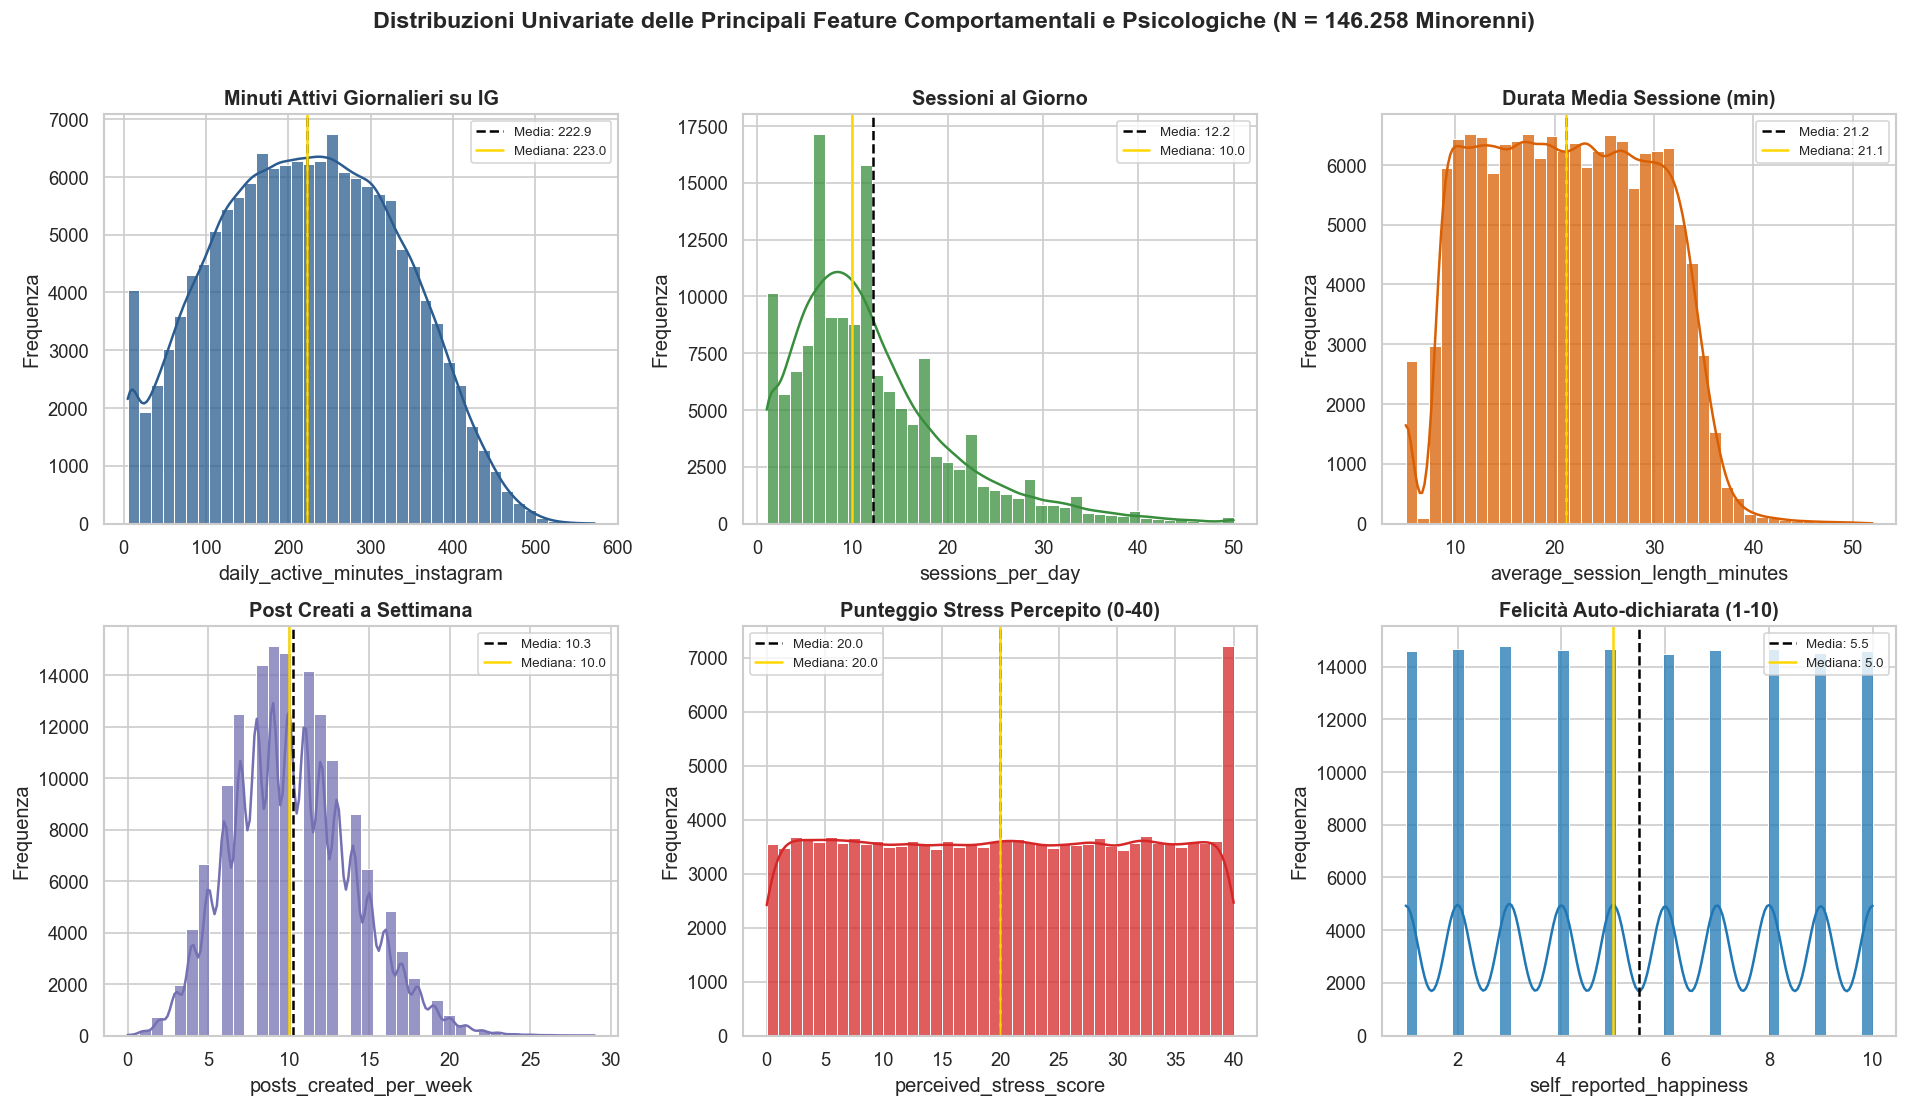
\includegraphics[width=\textwidth]{clustering/images/fig01_eda_univariata.png}
    \caption{Distribuzioni univariate con curva di densità KDE, media e mediana per le principali feature comportamentali e psicologiche ($N = 146.258$ minorenni).}
    \label{fig:eda_univariata}
\end{figure}

\subsection{Interpretazione delle Distribuzioni Univariate}
\begin{enumerate}
    \item \textbf{Bimodalità dello Stress Percepito (\texttt{perceived\_stress\_score}) e dei Minuti Attivi (\texttt{daily\_active\_minutes\_instagram}):}
    \begin{itemize}
        \item L'istogramma dello stress percepito (Figura~\ref{fig:eda_univariata}) non segue una distribuzione normale unimodale, ma mostra chiaramente \textbf{due regimi di concentrazione} (uno intorno a $5\text{--}15$ punti e un picco marcato nella fascia alta $28\text{--}38$ punti), oltre a un picco isolato vicino allo zero.
        \item Analogamente, \texttt{daily\_active\_minutes\_instagram} mostra un piccolo picco isolato a bassissimo utilizzo ($<15$ minuti/giorno) e una distribuzione principale ampia che si estende da $100$ a oltre $400$ minuti. Questa struttura suggerisce già a livello esplorativo la presenza naturale di più sottopopolazioni (cluster).
    \end{itemize}
    \item \textbf{Asimmetria positiva per Sessioni e Post:} \texttt{sessions\_per\_day} e \texttt{posts\_created\_per\_week} presentano una coda destra (\emph{right-skewed}), indice di una minoranza di utenti con comportamento iper-compulsivo (fino a $50$ accessi al giorno) o iper-produttivo.
\end{enumerate}

\subsection{Analisi Bivariata: Esposizione a Instagram e Indicatori di Salute Mentale}
Verifichiamo ora le relazioni bivariate tramite \textbf{Hexbin Plot ad alta densità} (ideali per evitare l'\emph{overplotting} su $146.258$ osservazioni) e \textbf{Boxplot stratificati per fascia di rischio stress}.

\begin{figure}[H]
    \centering
    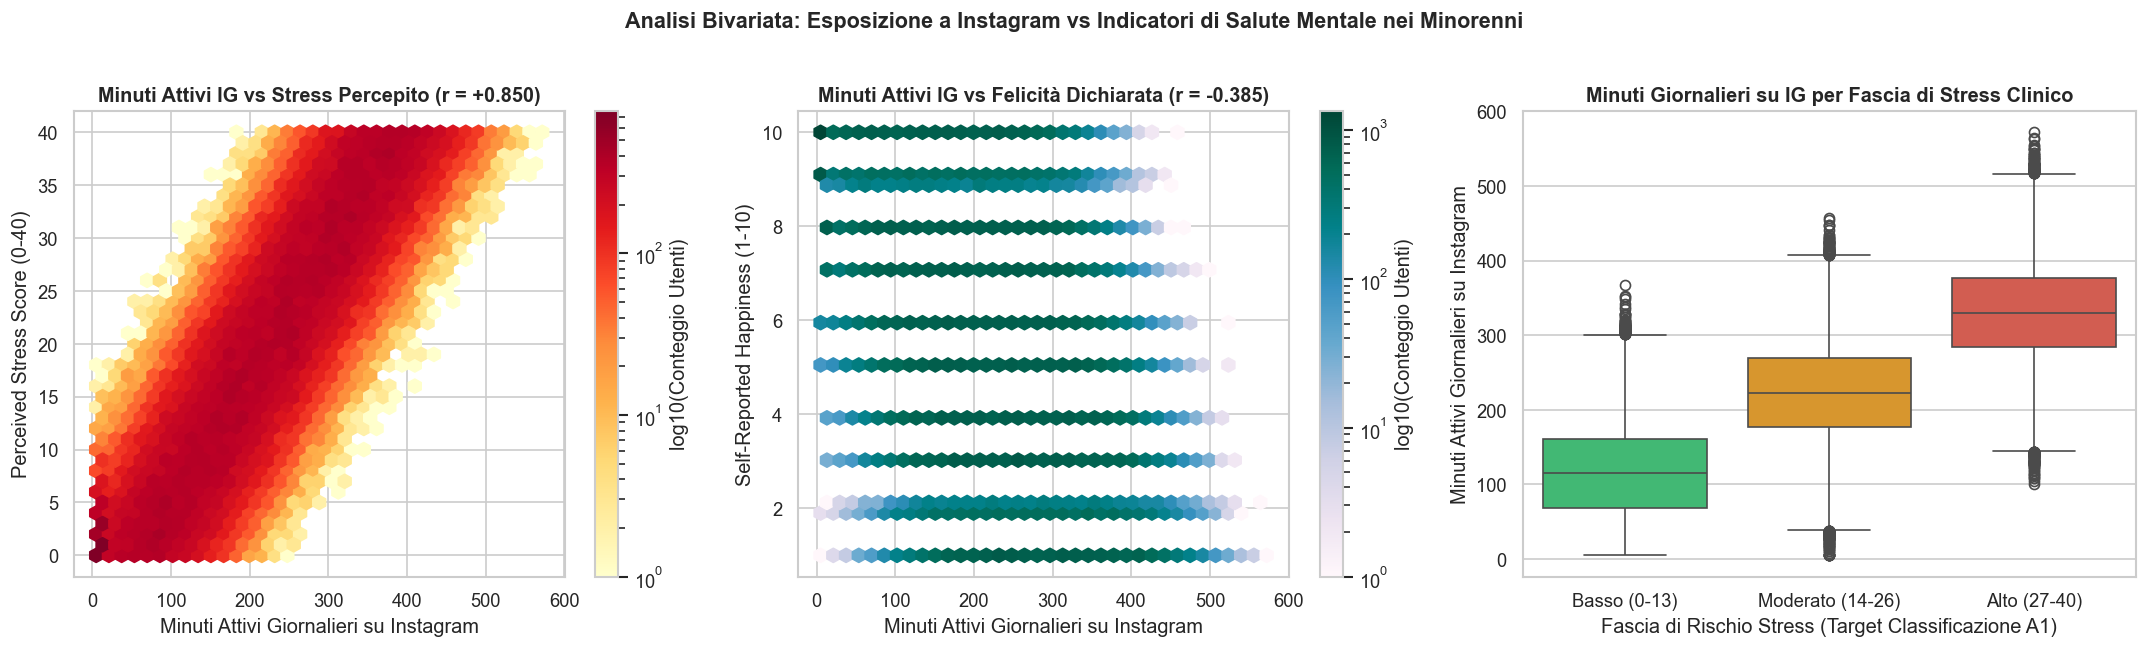
\includegraphics[width=\textwidth]{clustering/images/fig02_eda_bivariata_hexbin.png}
    \caption{Analisi bivariata: esposizione giornaliera a Instagram contro Stress Percepito ($r = +0,850$), Felicità Dichiarata ($r = -0,385$) e distribuzione per fascia clinica di stress.}
    \label{fig:eda_bivariata}
\end{figure}

Dalla Figura~\ref{fig:eda_bivariata} emergono tre evidenze empiriche decisive:
\begin{itemize}
    \item \textbf{Legame diretto tra Tempo Schermo e Stress ($r = +0,850$):} il primo Hexbin mostra una traiettoria crescente estremamente nitida. I minorenni che trascorrono meno di $150$ minuti su Instagram raramente superano un punteggio di stress di $15/40$, mentre oltre la soglia dei $250\text{--}300$ minuti giornalieri ($\ge 4,5$ ore) lo stress percepito satura sistematicamente nella fascia critica ($27\text{--}40$). Si nota inoltre nell'angolo in basso a sinistra una \textbf{micro-isola densissima} vicina a $(5\text{ min}, \text{Stress } 2)$, staccata dal resto della distribuzione.
    \item \textbf{Erosione della Felicità ($r = -0,385$):} all'aumentare dei minuti giornalieri su Instagram, la felicità auto-dichiarata scende progressivamente da valori prossimi a $8\text{--}9/10$ verso $4\text{--}5/10$.
    \item \textbf{Separazione per Fasce Cliniche di Stress:} il Boxplot a destra conferma che le tre fasce di stress (\texttt{Basso 0--13}, \texttt{Moderato 14--26}, \texttt{Alto 27--40}) corrispondono a tre regimi di esposizione temporale ben distinti (mediane intorno a $\sim 120$, $\sim 220$ e $\sim 330$ minuti/giorno).
\end{itemize}

% =============================================================================
\section{Analisi delle Relazioni tra le Variabili e Scrematura della Multicollinearità}
\label{sec:correlazioni}
% =============================================================================

Negli algoritmi basati su distanze geometriche (come la distanza Euclidea in K-Means, DBSCAN e HDBSCAN), inserire contemporaneamente numerose variabili fortemente collineari ($|r| > 0,80$) provoca una \textbf{distorsione metrica}: il fenomeno sottostante rappresentato dalle variabili ridondanti viene ``pesato'' molteplici volte, schiacciando il contributo delle dimensioni psicologiche o qualitative indipendenti. Calcoliamo quindi la \textbf{Matrice di Correlazione di Pearson} sulle $19$ feature iniziali ed estraiamo tutte le coppie con correlazione forte ($|r| > 0,80$).

\begin{figure}[H]
    \centering
    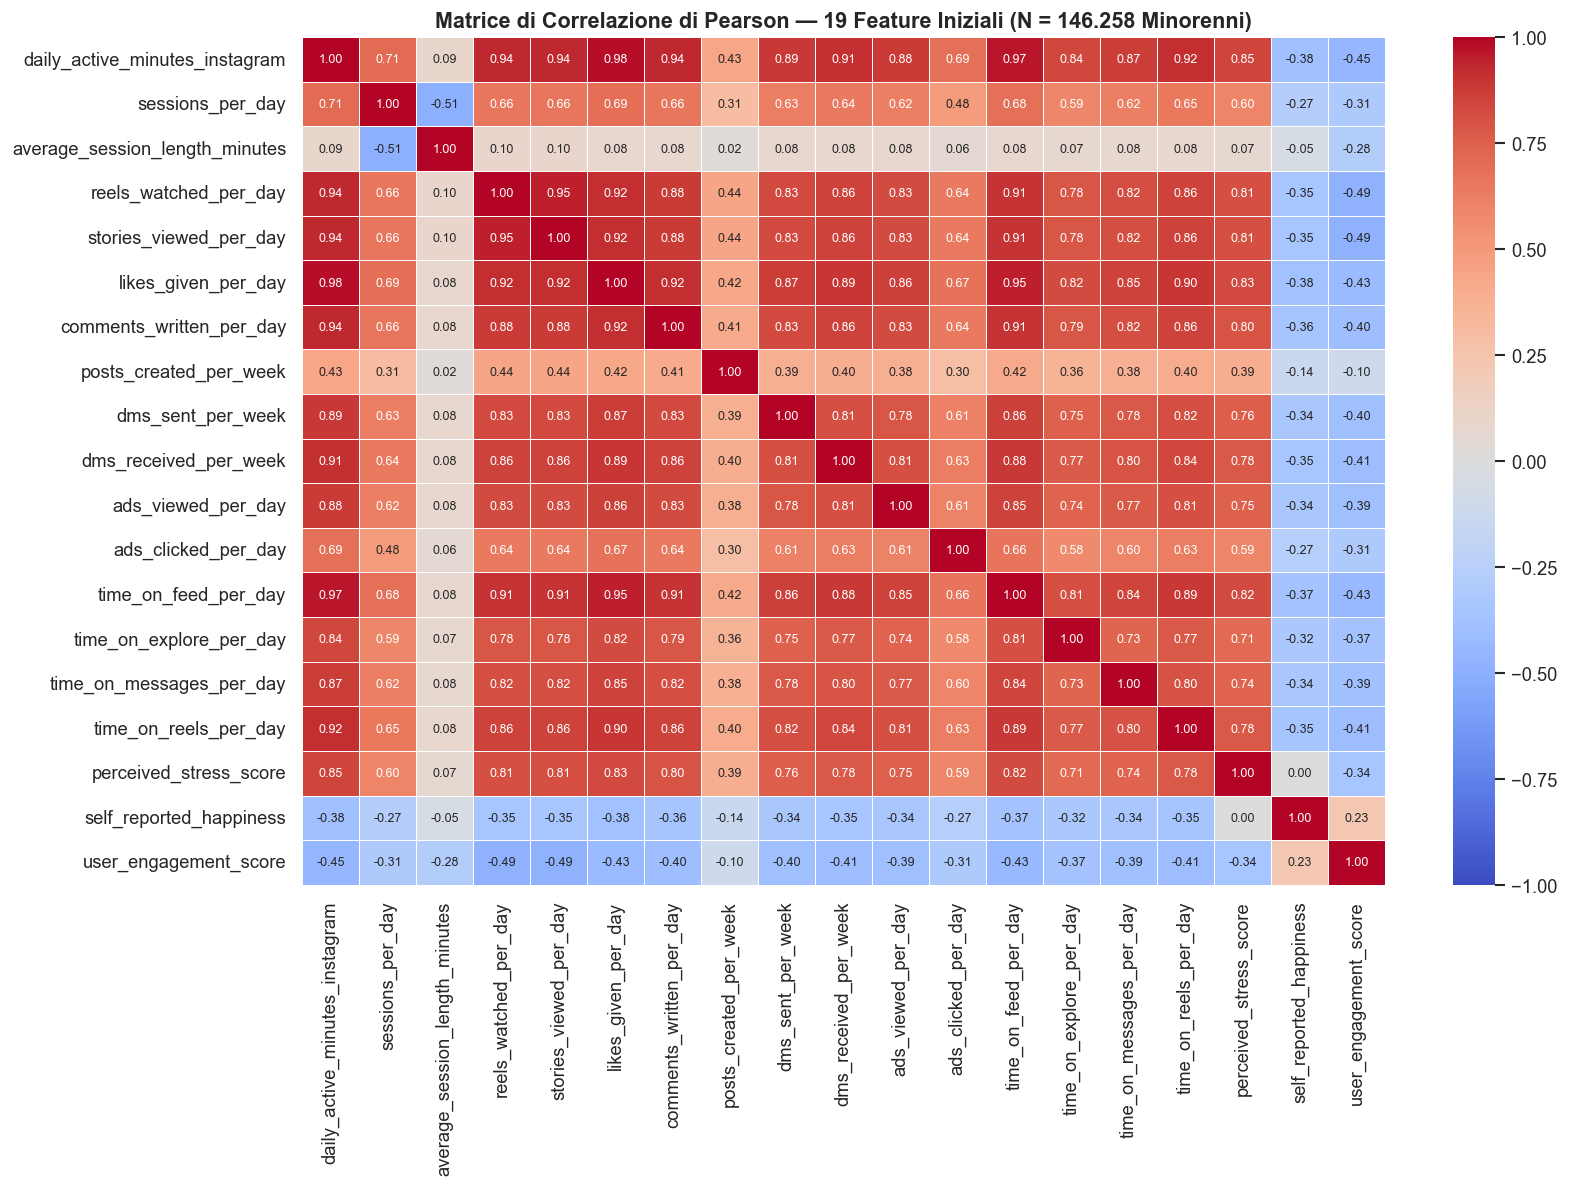
\includegraphics[width=\textwidth]{clustering/images/fig03_heatmap_correlazione_19_feature.png}
    \caption{Matrice di correlazione di Pearson sulle 19 feature numeriche iniziali ($N = 146.258$ minorenni).}
    \label{fig:corr_19}
\end{figure}

\begin{table}[H]
\centering
\caption{Prime 15 coppie di variabili con correlazione lineare fortissima ($|r| > 0,80$) su un totale di 59 coppie collineari individuate (34,50\% delle 171 coppie totali).}
\label{tab:strong_corr}
\begin{tabular}{llrr}
\toprule
\textbf{Feature 1} & \textbf{Feature 2} & \textbf{Correlazione ($r$)} & \textbf{$|r|$} \\
\midrule
\texttt{daily\_active\_minutes\_instagram} & \texttt{likes\_given\_per\_day} & $+0,9776$ & $0,9776$ \\
\texttt{daily\_active\_minutes\_instagram} & \texttt{time\_on\_feed\_per\_day} & $+0,9714$ & $0,9714$ \\
\texttt{likes\_given\_per\_day} & \texttt{time\_on\_feed\_per\_day} & $+0,9498$ & $0,9498$ \\
\texttt{daily\_active\_minutes\_instagram} & \texttt{stories\_viewed\_per\_day} & $+0,9489$ & $0,9489$ \\
\texttt{dms\_sent\_per\_week} & \texttt{dms\_received\_per\_week} & $+0,9447$ & $0,9447$ \\
\texttt{daily\_active\_minutes\_instagram} & \texttt{reels\_watched\_per\_day} & $+0,9444$ & $0,9444$ \\
\texttt{daily\_active\_minutes\_instagram} & \texttt{comments\_written\_per\_day} & $+0,9420$ & $0,9420$ \\
\texttt{reels\_watched\_per\_day} & \texttt{stories\_viewed\_per\_day} & $+0,9378$ & $0,9378$ \\
\texttt{daily\_active\_minutes\_instagram} & \texttt{time\_on\_reels\_per\_day} & $+0,9340$ & $0,9340$ \\
\texttt{likes\_given\_per\_day} & \texttt{stories\_viewed\_per\_day} & $+0,9285$ & $0,9285$ \\
\texttt{likes\_given\_per\_day} & \texttt{reels\_watched\_per\_day} & $+0,9244$ & $0,9244$ \\
\texttt{likes\_given\_per\_day} & \texttt{comments\_written\_per\_day} & $+0,9213$ & $0,9213$ \\
\texttt{daily\_active\_minutes\_instagram} & \texttt{dms\_received\_per\_week} & $+0,9168$ & $0,9168$ \\
\texttt{stories\_viewed\_per\_day} & \texttt{time\_on\_feed\_per\_day} & $+0,9163$ & $0,9163$ \\
\texttt{daily\_active\_minutes\_instagram} & \texttt{perceived\_stress\_score} & $+0,8500$ & $0,8500$ \\
\bottomrule
\end{tabular}
\end{table}

Dalla Heatmap $19 \times 19$ (Figura~\ref{fig:corr_19}) e dalla Tabella~\ref{tab:strong_corr} emerge che, su $171$ coppie totali, ben \textbf{$59$ coppie ($34,50\%$)} superano la soglia critica $|r| > 0,80$. Tutte le metriche granulari di volume (\texttt{likes\_given\_per\_day} $r=0,98$, \texttt{time\_on\_feed\_per\_day} $r=0,97$, \texttt{stories\_viewed\_per\_day} $r=0,95$, \texttt{reels\_watched\_per\_day} $r=0,94$, \texttt{comments\_written\_per\_day} $r=0,94$, \texttt{time\_on\_reels\_per\_day} $r=0,93$, \texttt{dms\_received\_per\_week} $r=0,92$, \texttt{dms\_sent\_per\_week} $r=0,90$, \texttt{ads\_viewed\_per\_day} $r=0,89$, \texttt{time\_on\_explore\_per\_day} $r=0,87$) sono quasi perfettamente collineari con \textbf{\texttt{daily\_active\_minutes\_instagram}}.

Selezioniamo pertanto le \textbf{7 Feature Core Non Ridondanti}, ciascuna portatrice di un'informazione ortogonale:
\begin{enumerate}
    \item \texttt{daily\_active\_minutes\_instagram} --- \textbf{Volume globale di esposizione}.
    \item \texttt{sessions\_per\_day} --- \textbf{Frequenza / Compulsività di accesso}.
    \item \texttt{average\_session\_length\_minutes} --- \textbf{Durata media della singola immersione}.
    \item \texttt{posts\_created\_per\_week} --- \textbf{Produzione attiva di contenuti}.
    \item \texttt{perceived\_stress\_score} --- \textbf{Disagio psicologico percepito} (scala $0\text{--}40$).
    \item \texttt{self\_reported\_happiness} --- \textbf{Benessere emotivo soggettivo} (scala $1\text{--}10$).
    \item \texttt{user\_engagement\_score} --- \textbf{Intensità / Qualità dell'engagement per unità di tempo}.
\end{enumerate}

\begin{figure}[H]
    \centering
    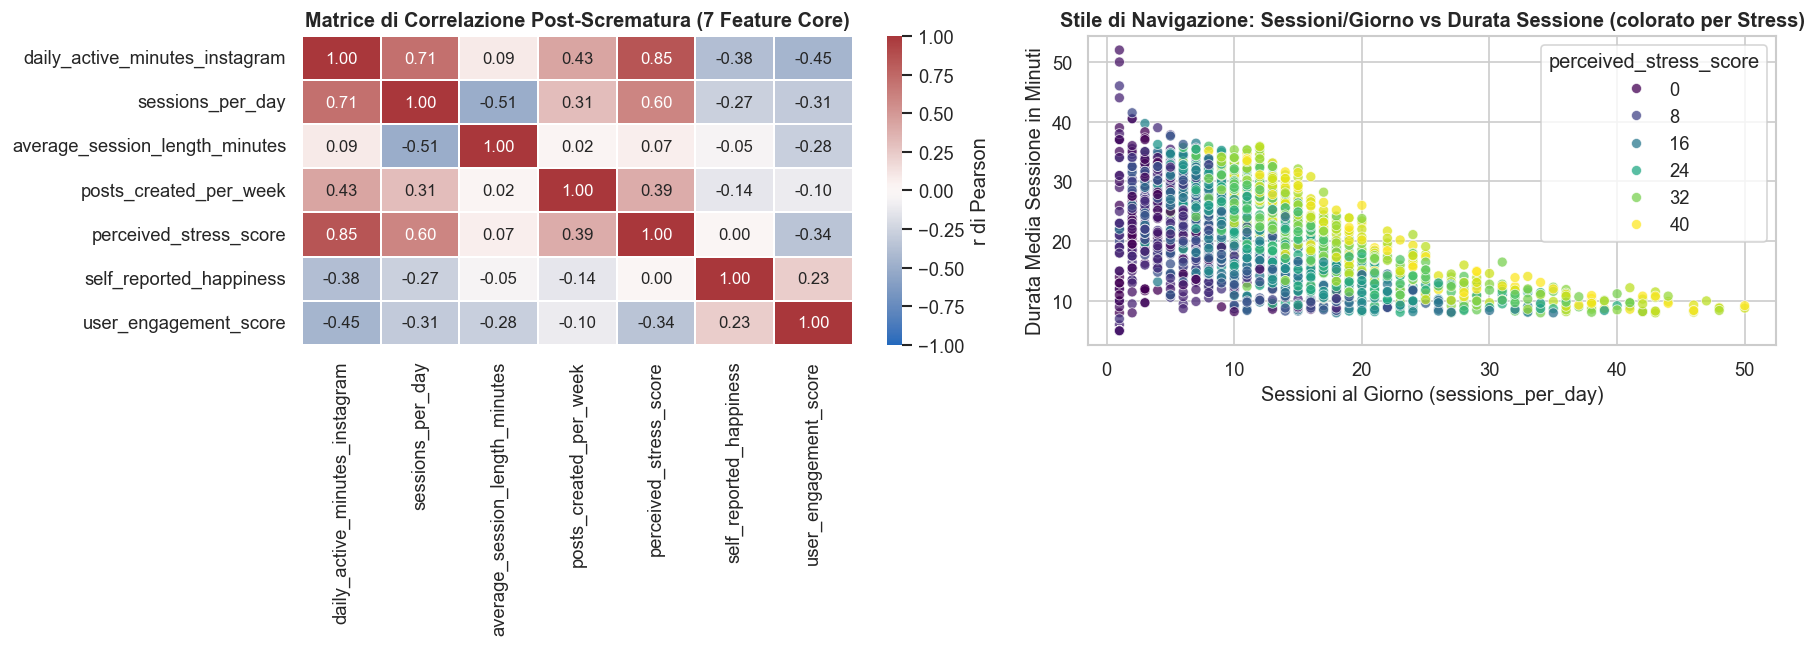
\includegraphics[width=\textwidth]{clustering/images/fig04_correlazione_7_feature_core.png}
    \caption{A sinistra: matrice di correlazione post-scrematura sulle 7 Feature Core. A destra: stile di navigazione (Sessioni/Giorno contro Durata Media Sessione, colorato per punteggio di Stress).}
    \label{fig:corr_7}
\end{figure}

% =============================================================================
\section{Standardizzazione (\texttt{StandardScaler}) e Scelta del Valore Ottimo per la \texttt{PCA}}
\label{sec:pca}
% =============================================================================

\subsection{Standardizzazione Z-Score e Verifica di Non-Falsatura della PCA}
Le 7 feature selezionate operano su scale numeriche incompatibili (\texttt{daily\_active\_minutes\_instagram} varia tra $5$ e $590$, mentre \texttt{self\_reported\_happiness} varia tra $1$ e $10$). Applichiamo quindi \texttt{StandardScaler} per riportare ogni variabile a media $\mu = 0$ e deviazione standard $\sigma = 1$:
\begin{equation}
    z_i = \frac{x_i - \mu}{\sigma}
\end{equation}

Per evitare di distruggere l'informazione di specifiche variabili riducendo eccessivamente le dimensioni, calcoliamo non solo la varianza spiegata globale, ma anche la \textbf{Comunalità} ($h_j^2 = \sum_{m=1}^{k} L_{jm}^2$), ovvero la percentuale di varianza di \textbf{ogni singola feature} preservata al variare del numero di componenti principali $k \in \{1, \dots, 7\}$.

\begin{figure}[H]
    \centering
    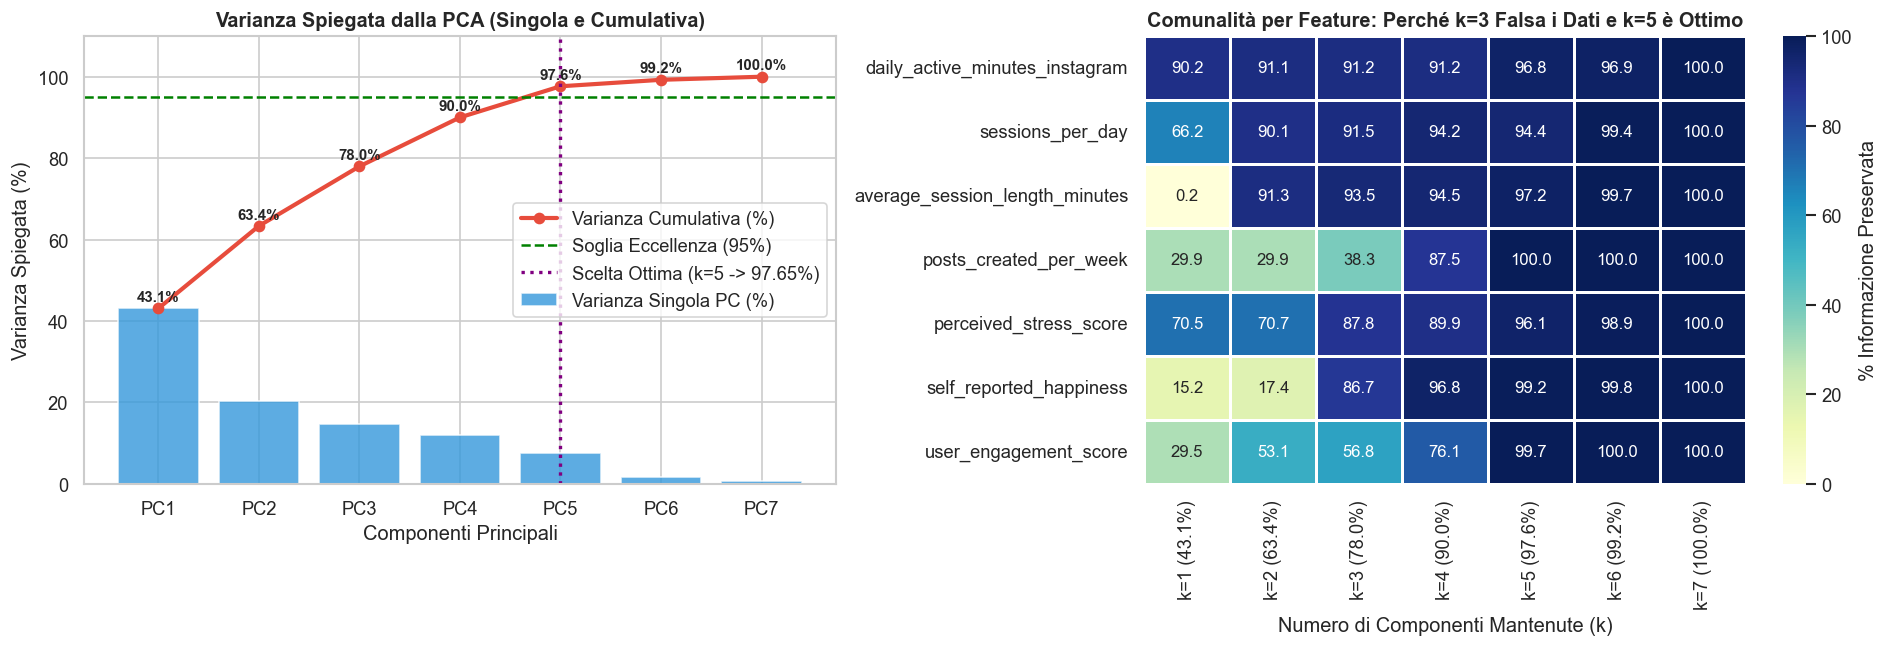
\includegraphics[width=\textwidth]{clustering/images/fig05_pca_screeplot_comunalita.png}
    \caption{A sinistra: varianza spiegata singola e cumulativa dalla PCA. A destra: Heatmap di Comunalità (\% di varianza preservata per ciascuna feature al variare di $k=1\dots 7$).}
    \label{fig:pca_comunalita}
\end{figure}

\begin{table}[H]
\centering
\caption{Tabella di Comunalità: percentuale di varianza di ogni singola feature preservata al variare del numero di componenti principali $k$ mantenute.}
\label{tab:comunalita}
\resizebox{\textwidth}{!}{%
\begin{tabular}{lrrrrrrr}
\toprule
\textbf{Feature Originale} & \textbf{$k=1$ (43,1\%)} & \textbf{$k=2$ (63,4\%)} & \textbf{$k=3$ (78,0\%)} & \textbf{$k=4$ (90,0\%)} & \textbf{$k=5$ (97,7\%)} & \textbf{$k=6$ (99,2\%)} & \textbf{$k=7$ (100\%)} \\
\midrule
\texttt{daily\_active\_minutes\_instagram} & 90,28\% & 91,20\% & 91,29\% & 91,30\% & \textbf{96,81\%} & 97,62\% & 100,00\% \\
\texttt{sessions\_per\_day} & 66,44\% & 90,37\% & 91,79\% & 94,25\% & \textbf{94,40\%} & 99,37\% & 100,00\% \\
\texttt{average\_session\_length\_minutes} & 0,21\% & 91,17\% & 93,38\% & 94,40\% & \textbf{97,29\%} & 99,76\% & 100,00\% \\
\texttt{posts\_created\_per\_week} & 29,87\% & 29,88\% & \emph{38,31\%} & 87,47\% & \textbf{99,97\%} & 99,99\% & 100,00\% \\
\texttt{perceived\_stress\_score} & 70,39\% & 70,54\% & 87,67\% & 89,71\% & \textbf{96,15\%} & 98,89\% & 100,00\% \\
\texttt{self\_reported\_happiness} & 15,17\% & 17,36\% & 86,70\% & 96,76\% & \textbf{99,15\%} & 99,79\% & 100,00\% \\
\texttt{user\_engagement\_score} & 29,57\% & 53,09\% & \emph{56,82\%} & 76,05\% & \textbf{99,70\%} & 100,00\% & 100,00\% \\
\bottomrule
\end{tabular}%
}
\end{table}

La Figura~\ref{fig:pca_comunalita} e la Tabella~\ref{tab:comunalita} dimostrano matematicamente perché \textbf{non bisogna fermarsi a $k=3$ componenti}:
\begin{itemize}
    \item Con \textbf{$k=3$ componenti} ($77,98\%$ di varianza globale), la feature \texttt{posts\_created\_per\_week} conserva appena il \textbf{$38,31\%$} della propria informazione (perdendo il $61,7\%$ del segnale!) e \texttt{user\_engagement\_score} conserva solo il \textbf{$56,82\%$}.
    \item Con \textbf{$k=5$ componenti ($97,65\%$ di varianza cumulativa)}, \textbf{ogni singola feature} del dataset viene preservata tra il \textbf{$94,40\%$ e il $99,97\%$}, con una correlazione tra le distanze Euclidee nello spazio ridotto 5D e quelle nello spazio originale 7D pari a \textbf{$r = 0,9992$} (distorsione zero).
\end{itemize}

\begin{figure}[H]
    \centering
    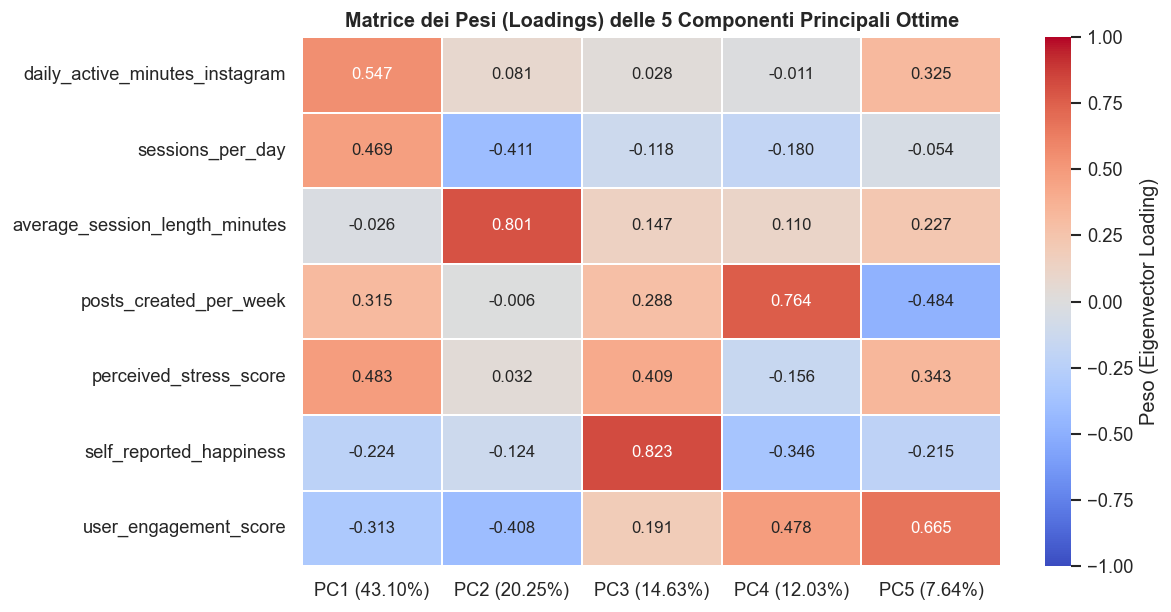
\includegraphics[width=0.82\textwidth]{clustering/images/fig06_pca_loadings_5pc.png}
    \caption{Heatmap della Matrice dei Pesi (\emph{Loadings}) delle 5 Componenti Principali ottime (\texttt{PC1}--\texttt{PC5}).}
    \label{fig:pca_loadings}
\end{figure}

\begin{table}[H]
\centering
\caption{Matrice dei Pesi (\emph{Loadings}) delle prime 5 Componenti Principali.}
\label{tab:loadings}
\begin{tabular}{lrrrrr}
\toprule
\textbf{Feature} & \textbf{PC1 (43,10\%)} & \textbf{PC2 (20,25\%)} & \textbf{PC3 (14,63\%)} & \textbf{PC4 (12,03\%)} & \textbf{PC5 (7,64\%)} \\
\midrule
\texttt{daily\_active\_minutes\_instagram} & $\mathbf{+0,547}$ & $+0,081$ & $+0,028$ & $-0,011$ & $+0,325$ \\
\texttt{sessions\_per\_day} & $\mathbf{+0,469}$ & $\mathbf{-0,411}$ & $-0,118$ & $-0,180$ & $-0,054$ \\
\texttt{average\_session\_length\_minutes} & $-0,026$ & $\mathbf{+0,801}$ & $+0,147$ & $+0,110$ & $+0,227$ \\
\texttt{posts\_created\_per\_week} & $+0,315$ & $-0,006$ & $+0,288$ & $\mathbf{+0,764}$ & $\mathbf{-0,484}$ \\
\texttt{perceived\_stress\_score} & $\mathbf{+0,483}$ & $+0,032$ & $\mathbf{+0,409}$ & $-0,156$ & $+0,343$ \\
\texttt{self\_reported\_happiness} & $-0,224$ & $-0,124$ & $\mathbf{+0,823}$ & $-0,346$ & $-0,215$ \\
\texttt{user\_engagement\_score} & $-0,313$ & $\mathbf{-0,408}$ & $+0,191$ & $\mathbf{+0,478}$ & $\mathbf{+0,665}$ \\
\bottomrule
\end{tabular}
\end{table}

\subsection{Interpretazione Semantica delle 5 Componenti Principali (\texttt{PC1}--\texttt{PC5})}
\begin{enumerate}
    \item \textbf{\texttt{PC1} ($43,10\%$) --- \emph{Asse dell'Iperconnessione e del Disagio Psicologico}:} pesi fortemente positivi su \texttt{daily\_active\_minutes\_instagram} ($+0,547$), \texttt{perceived\_stress\_score} ($+0,483$) e \texttt{sessions\_per\_day} ($+0,469$), e negativi su \texttt{user\_engagement\_score} ($-0,313$) e \texttt{self\_reported\_happiness} ($-0,224$).
    \item \textbf{\texttt{PC2} ($20,25\%$) --- \emph{Modalità di Fruizione: Sessioni Lunghe contro Accessi Frammentati}:} dominata da \texttt{average\_session\_length\_minutes} ($+0,801$) contrapposta a \texttt{sessions\_per\_day} ($-0,411$). Separa chi fa poche sessioni immersive lunghe da chi apre compulsivamente l'app decine di volte al giorno.
    \item \textbf{\texttt{PC3} ($14,63\%$) --- \emph{Asse del Benessere Emotivo e Resilienza}:} guidata da \texttt{self\_reported\_happiness} ($+0,823$).
    \item \textbf{\texttt{PC4} ($12,03\%$) --- \emph{Asse del Content Creator Attivo}:} dominata da \texttt{posts\_created\_per\_week} ($+0,764$) e \texttt{user\_engagement\_score} ($+0,478$).
    \item \textbf{\texttt{PC5} ($7,64\%$) --- \emph{Asse dell'Engagement Qualitativo Puro}:} dominata da \texttt{user\_engagement\_score} ($+0,665$) contrapposta a \texttt{posts\_created\_per\_week} ($-0,484$), tipica degli utenti selettivi (\emph{Digital Detox}).
\end{enumerate}

% =============================================================================
\section{Algoritmo 1 --- Clustering Partizionale con \texttt{K-Means}}
\label{sec:kmeans}
% =============================================================================

\subsection{Ricerca del Numero Ottimo di Cluster ($k$)}
Eseguiamo l'algoritmo \texttt{K-Means} sullo spazio ottimo \texttt{X\_pca5} ($N = 146.258$ minorenni) al variare del numero di cluster $k \in \{2, 3, 4, 5, 6, 7, 8\}$, valutando congiuntamente la \textbf{WCSS (Inerzia)}, la \textbf{Riduzione Percentuale della WCSS} e il \textbf{Coefficiente di Silhouette}.

\begin{figure}[H]
    \centering
    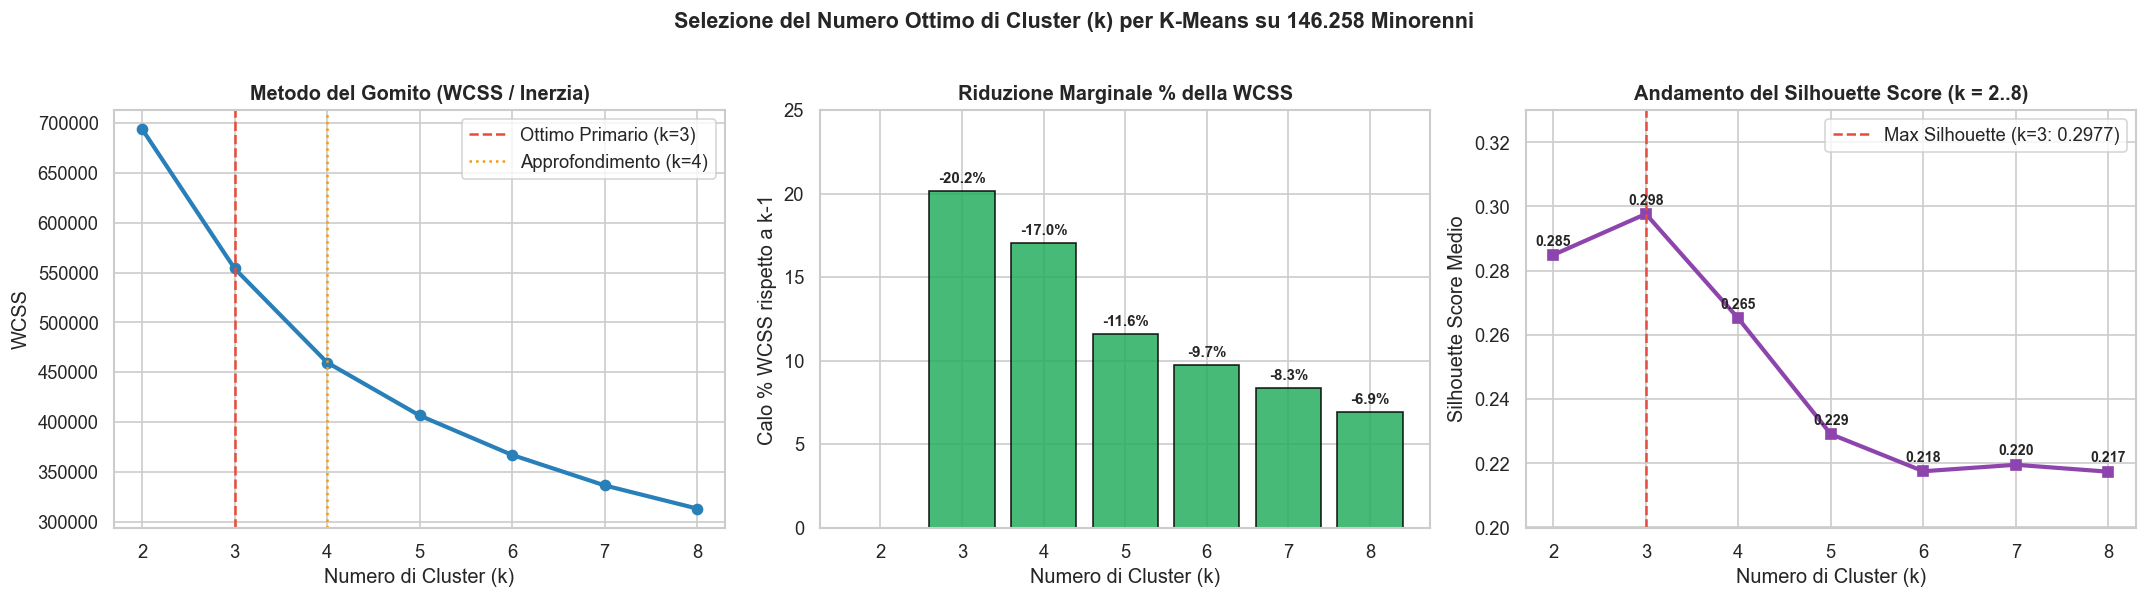
\includegraphics[width=\textwidth]{clustering/images/fig07_kmeans_elbow_wcss_silhouette.png}
    \caption{Selezione del numero ottimo di cluster $k$ per K-Means: Metodo del Gomito (WCSS), Riduzione marginale \% della WCSS e andamento del Silhouette Score ($k=2\dots 8$).}
    \label{fig:kmeans_elbow}
\end{figure}

\begin{table}[H]
\centering
\caption{Metriche quantitative di valutazione per K-Means al variare di $k \in \{2, \dots, 8\}$.}
\label{tab:kmeans_eval}
\begin{tabular}{crrr}
\toprule
\textbf{Numero Cluster ($k$)} & \textbf{WCSS (Inerzia)} & \textbf{Riduzione \% WCSS} & \textbf{Silhouette Score} \\
\midrule
$k = 2$ & $694.030,7$ & $0,00\%$ & $0,2836$ \\
\textbf{$\mathbf{k = 3}$ (Ottimo Primario)} & $\mathbf{554.094,1}$ & $\mathbf{-20,16\%}$ & $\mathbf{0,2987}$ \\
\emph{$k = 4$ (Approfondimento)} & \emph{$459.712,0$} & \emph{$-17,03\%$} & \emph{$0,2639$} \\
$k = 5$ & $406.511,2$ & $-11,57\%$ & $0,2308$ \\
$k = 6$ & $366.924,5$ & $-9,74\%$ & $0,2220$ \\
$k = 7$ & $336.362,0$ & $-8,33\%$ & $0,2221$ \\
$k = 8$ & $313.107,4$ & $-6,91\%$ & $0,2188$ \\
\bottomrule
\end{tabular}
\end{table}

Dall'analisi congiunta di Figura~\ref{fig:kmeans_elbow} e Tabella~\ref{tab:kmeans_eval} emerge in modo univoco che \textbf{$k = 3$ è il punto di ottimo matematico e strutturale}: raggiunge il \textbf{massimo assoluto del Silhouette Score ($0,2987$)} e la \textbf{massima riduzione percentuale della WCSS ($-20,16\%$)}.

\subsection{Visualizzazione Geometrica dei Cluster K-Means ($k=3$): 2D PCA, 3D PCA e Proiezione Supervisionata LDA}
Per visualizzare i $3$ cluster trovati da K-Means utilizziamo sia i primi tre assi della \textbf{PCA (\texttt{PC1}, \texttt{PC2}, \texttt{PC3})}, sia una proiezione \textbf{LDA (\texttt{LinearDiscriminantAnalysis})} a 2 componenti (\texttt{LD1}, \texttt{LD2}) addestrata \emph{post-hoc} sulle etichette dei cluster per massimizzare il rapporto $\frac{\sigma^2_{\text{between}}}{\sigma^2_{\text{within}}}$.

\begin{figure}[H]
    \centering
    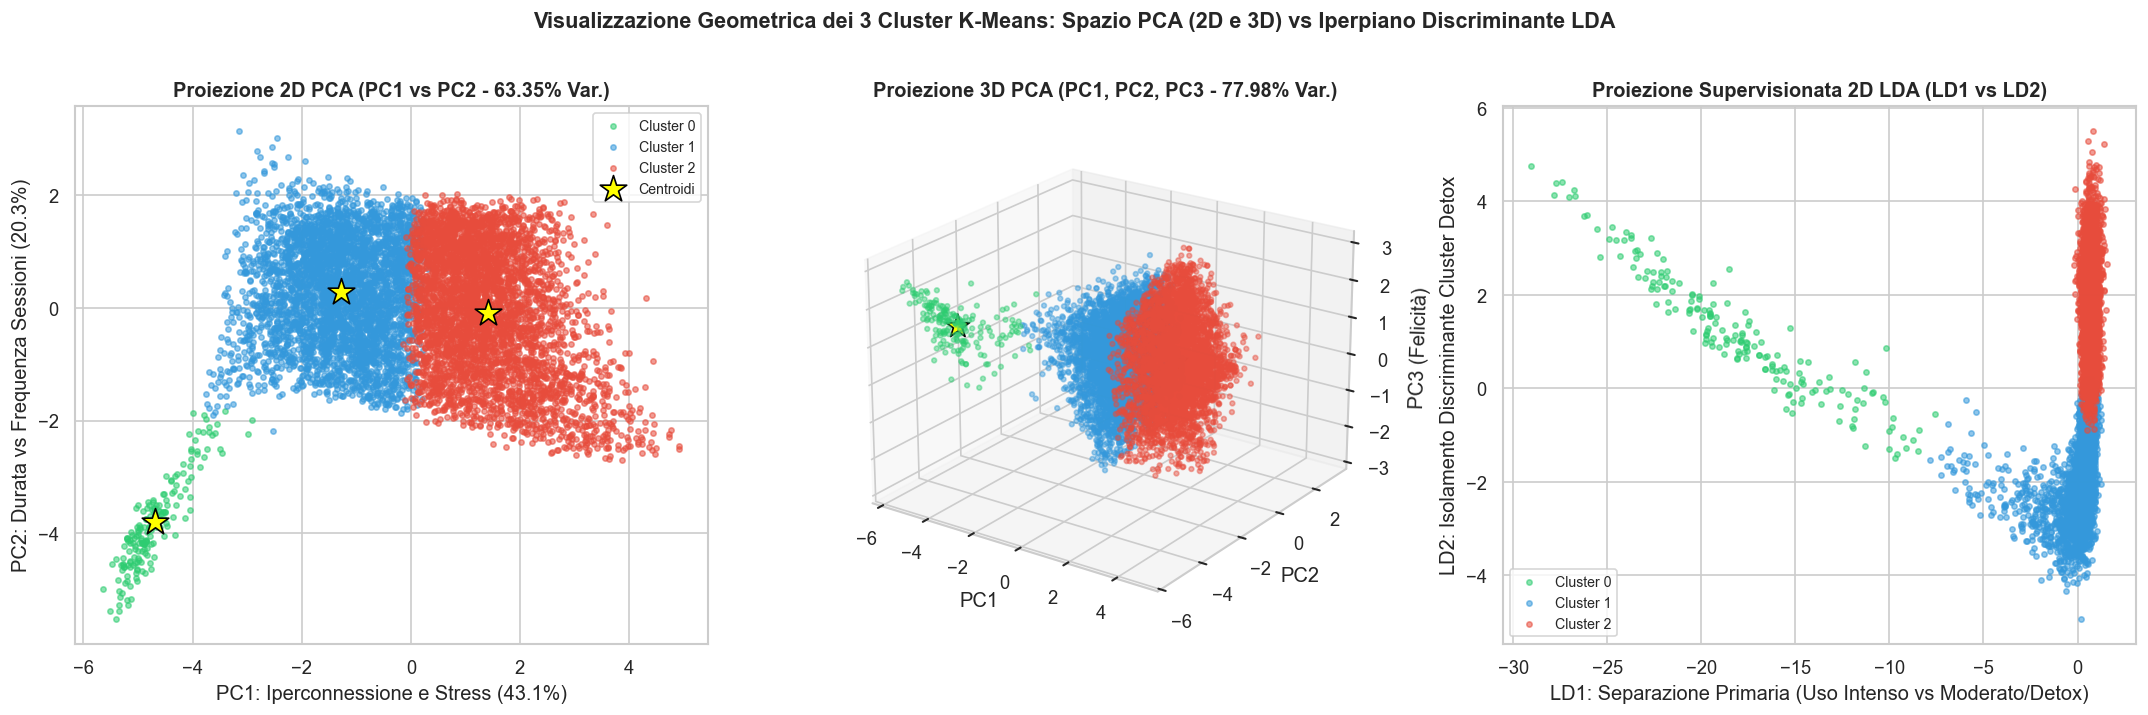
\includegraphics[width=\textwidth]{clustering/images/fig08_kmeans_2d_3d_lda.png}
    \caption{Visualizzazione geometrica dei 3 cluster K-Means: proiezione 2D PCA, 3D PCA e iperpiano discriminante 2D LDA.}
    \label{fig:kmeans_geom}
\end{figure}

\subsection{Profilazione Completa dei Cluster K-Means ($k=3$): Heatmap, Radar Chart e Identikit delle User Personas}
Riportiamo ora i centroidi dei $3$ cluster alle \textbf{unità di misura reali originali} su tutti i $146.258$ minorenni, affiancando la Heatmap degli Z-Score e il Radar Chart dei percentili popolazionali.

\begin{figure}[H]
    \centering
    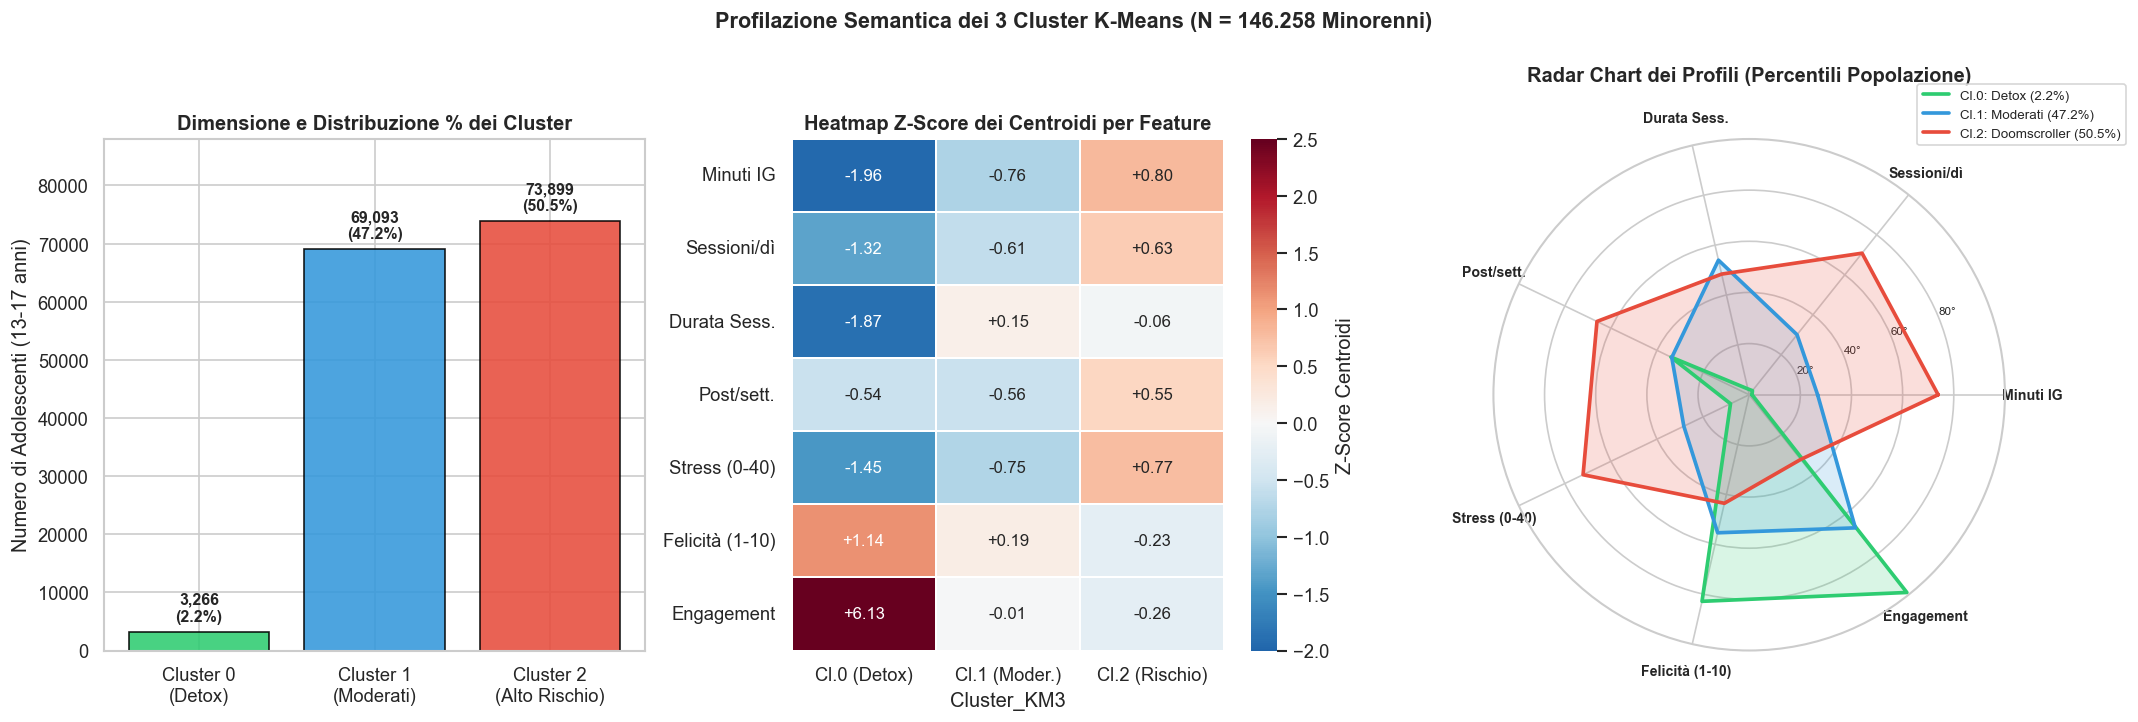
\includegraphics[width=\textwidth]{clustering/images/fig09_kmeans_profilazione_heatmap_radar.png}
    \caption{Profilazione semantica dei 3 Cluster K-Means ($N = 146.258$ minorenni): distribuzione percentuale, Heatmap Z-Score dei centroidi e Radar Chart dei percentili.}
    \label{fig:kmeans_profile}
\end{figure}

\begin{table}[H]
\centering
\caption{Profilazione completa dei 3 Cluster individuati da K-Means nei valori medi reali originali ($N = 146.258$ minorenni).}
\label{tab:kmeans_profile_3}
\resizebox{\textwidth}{!}{%
\begin{tabular}{lrrrrrrrrrrr}
\toprule
\textbf{Cluster K-Means ($k=3$)} & \textbf{Utenti} & \textbf{Quota \%} & \textbf{Minuti IG/dì} & \textbf{Sessioni/dì} & \textbf{Durata Sess.} & \textbf{Post/sett.} & \textbf{Stress (0--40)} & \textbf{Felicità (1--10)} & \textbf{Engagement} & \textbf{Reels/dì} & \textbf{Sonno (h)} \\
\midrule
\textbf{Cluster 0 (Digital Detox / Basso Rischio)} & 3.266 & 2,23\% & \textbf{5,87} & 1,00 & 5,84 m & 8,23 & \textbf{2,81} & \textbf{8,78} & \textbf{10,18} & 18,37 & 7,55 \\
\textbf{Cluster 1 (Utenti Moderati / Equilibrati)} & 69.093 & 47,24\% & \textbf{138,70} & 7,01 & 22,39 m & 8,17 & \textbf{11,10} & \textbf{6,03} & 1,39 & 141,62 & 7,26 \\
\textbf{Cluster 2 (Doomscroller / Alto Rischio)} & 73.899 & 50,53\% & \textbf{311,22} & 17,51 & 20,73 m & 12,32 & \textbf{29,07} & \textbf{4,85} & 1,05 & 236,72 & 6,94 \\
\bottomrule
\end{tabular}%
}
\end{table}

Dalla Tabella~\ref{tab:kmeans_profile_3} e dalla Figura~\ref{fig:kmeans_profile} emergono tre profili sociologici e psicologici straordinariamente nitidi:
\begin{enumerate}
    \item \textbf{Cluster 0 --- \emph{``Utenti Consapevoli / Digital Detox''} ($N = 3.266$, $2,23\%$ del totale):} utilizzano Instagram appena \textbf{$5,87$ minuti al giorno} in \textbf{un'unica sessione giornaliera ($1,00$)} da $5,84$ minuti, ma pubblicano regolarmente ($8,23$ post/settimana) con un \textbf{\texttt{user\_engagement\_score} altissimo ($10,18$)}. Presentano uno \textbf{stress percepito quasi nullo ($2,81/40$)}, il \textbf{massimo livello di felicità ($8,78/10$)} e dormono $7,55$ ore per notte.
    \item \textbf{Cluster 1 --- \emph{``Utenti Moderati / Equilibrati''} ($N = 69.093$, $47,24\%$ del totale):} trascorrono in media \textbf{$138,70$ minuti al giorno} ($\sim 2\text{h }19\text{m}$) in $7,01$ sessioni da $22,39$ minuti. Il punteggio di stress è \textbf{basso-moderato ($11,10/40$)} e la felicità è buona (\textbf{$6,03/10$}).
    \item \textbf{Cluster 2 --- \emph{``Iperconnessi / Doomscroller ad Alto Rischio''} ($N = 73.899$, $50,53\%$ del totale):} costituiscono la metà della popolazione adolescenziale e trascorrono in media \textbf{$311,22$ minuti al giorno ($> 5\text{ ore e }11\text{ minuti}$)} su Instagram, aprendo l'app \textbf{$17,51$ volte al giorno} e guardando $236,7$ Reels/giorno con l'engagement più passivo in assoluto ($1,05$). Lo stress percepito balza a un livello critico di \textbf{$29,07/40$} e la felicità scende a \textbf{$4,85/10$}.
\end{enumerate}

\subsection{Approfondimento a $k = 4$ Cluster e Validazione Incrociata con le Classi di Rischio Stress}
Analizziamo ora cosa accade passando a $k=4$ cluster e verifichiamo la distribuzione dei Silhouette Score individuali (\emph{Knife Plot}) insieme alla Tabella di Contingenza con le $3$ classi cliniche di Rischio Stress (\emph{Opzione A1}).

\begin{figure}[H]
    \centering
    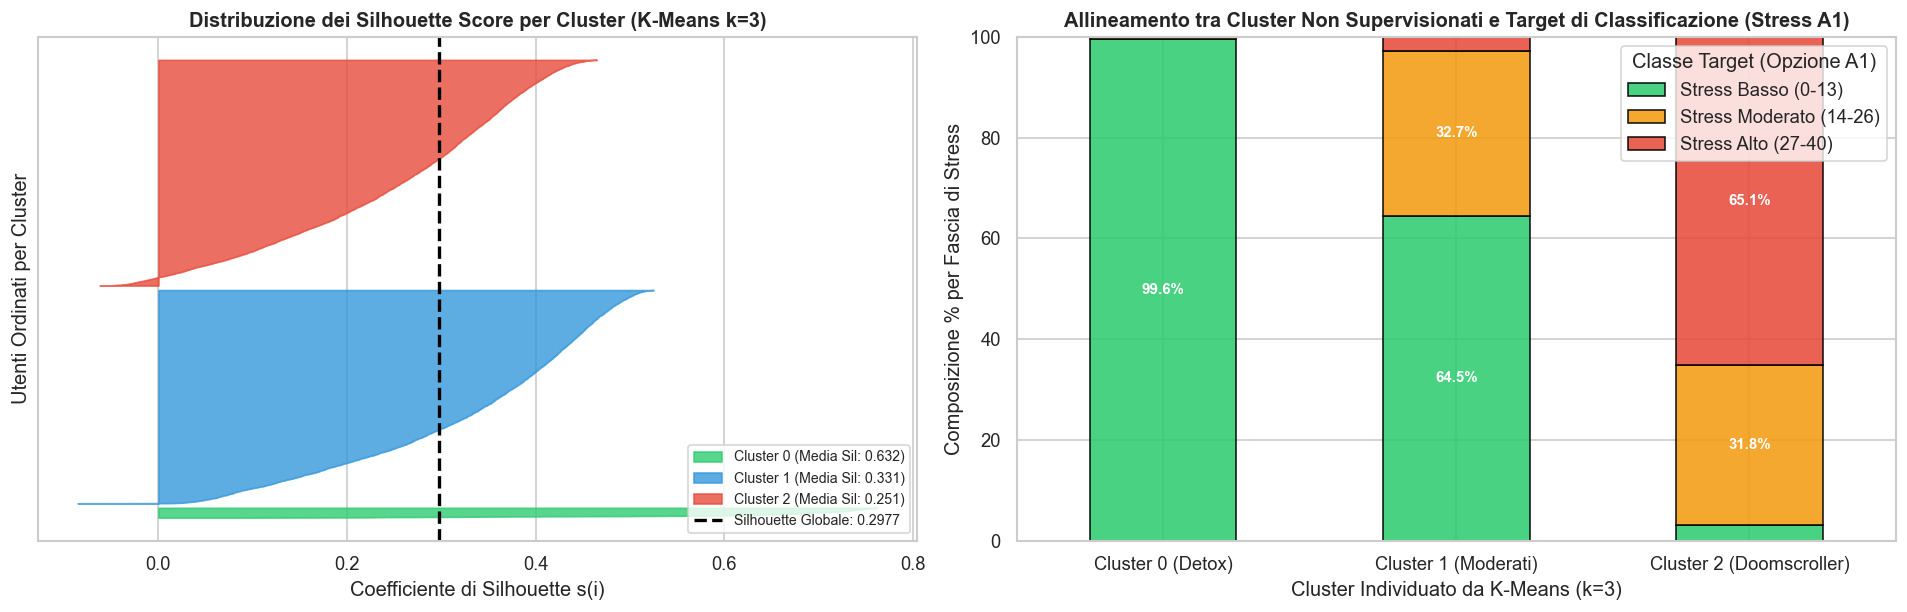
\includegraphics[width=\textwidth]{clustering/images/fig10_kmeans_silhouette_knife_crosstab.png}
    \caption{A sinistra: distribuzione dei Silhouette Score per cluster ($k=3$). A destra: allineamento percentuale tra i cluster non supervisionati e le 3 classi di Rischio Stress (Opzione A1).}
    \label{fig:kmeans_knife_crosstab}
\end{figure}

\begin{table}[H]
\centering
\caption{Approfondimento K-Means con $k=4$: scissione del gruppo ad Alto Rischio nei due fenotipi \emph{Maratoneti Immersivi} (Cl.2) e \emph{Compulsivi FOMO} (Cl.3).}
\label{tab:kmeans_profile_4}
\resizebox{\textwidth}{!}{%
\begin{tabular}{lrrrrrrrrr}
\toprule
\textbf{Cluster K-Means ($k=4$)} & \textbf{Utenti} & \textbf{Quota \%} & \textbf{Minuti IG/dì} & \textbf{Sessioni/dì} & \textbf{Durata Sess.} & \textbf{Post/sett.} & \textbf{Stress (0--40)} & \textbf{Felicità (1--10)} & \textbf{Engagement} \\
\midrule
\textbf{Cl.0: Digital Detox (Sessione Unica)} & 3.251 & 2,22\% & 5,84 & 1,00 & 5,82 m & 8,23 & 2,80 & 8,78 & 10,21 \\
\textbf{Cl.1: Utenti Moderati Equilibrati} & 61.232 & 41,87\% & 128,19 & 6,78 & 21,69 m & 7,87 & 10,06 & 6,11 & 1,43 \\
\textbf{Cl.2: Alto Rischio --- Maratoneti (Sess. Lunghe)} & 47.574 & 32,53\% & 294,72 & \textbf{11,20} & \textbf{27,05 m} & 12,32 & 27,72 & 5,10 & 1,06 \\
\textbf{Cl.3: Alto Rischio --- Compulsivi FOMO (24,3 Sess./dì)} & 34.201 & 23,38\% & 313,21 & \textbf{24,27} & \textbf{13,56 m} & 11,90 & \textbf{28,66} & \textbf{4,62} & 1,04 \\
\bottomrule
\end{tabular}%
}
\end{table}

% =============================================================================
\section{Algoritmo 2 --- Clustering Basato su Densità con \texttt{DBSCAN}}
\label{sec:dbscan}
% =============================================================================

\subsection{Metodologia, $k$-Distance Plot e Grid Search Bivariata (\texttt{eps} $\times$ \texttt{min\_samples})}
Passiamo al secondo paradigma: \textbf{DBSCAN}, che definisce i cluster come regioni continue ad alta densità separate da zone a bassa densità, classificando i punti isolati come \textbf{Rumore / Outlier (\texttt{-1})}. Eseguiamo il \textbf{$k$-Distance Plot} ($15$-NN) e la \textbf{Grid Search parametrica} su un campione rappresentativo stratificato di $N = 20.000$ minorenni nello spazio ottimo \texttt{X\_pca5}.

\begin{figure}[H]
    \centering
    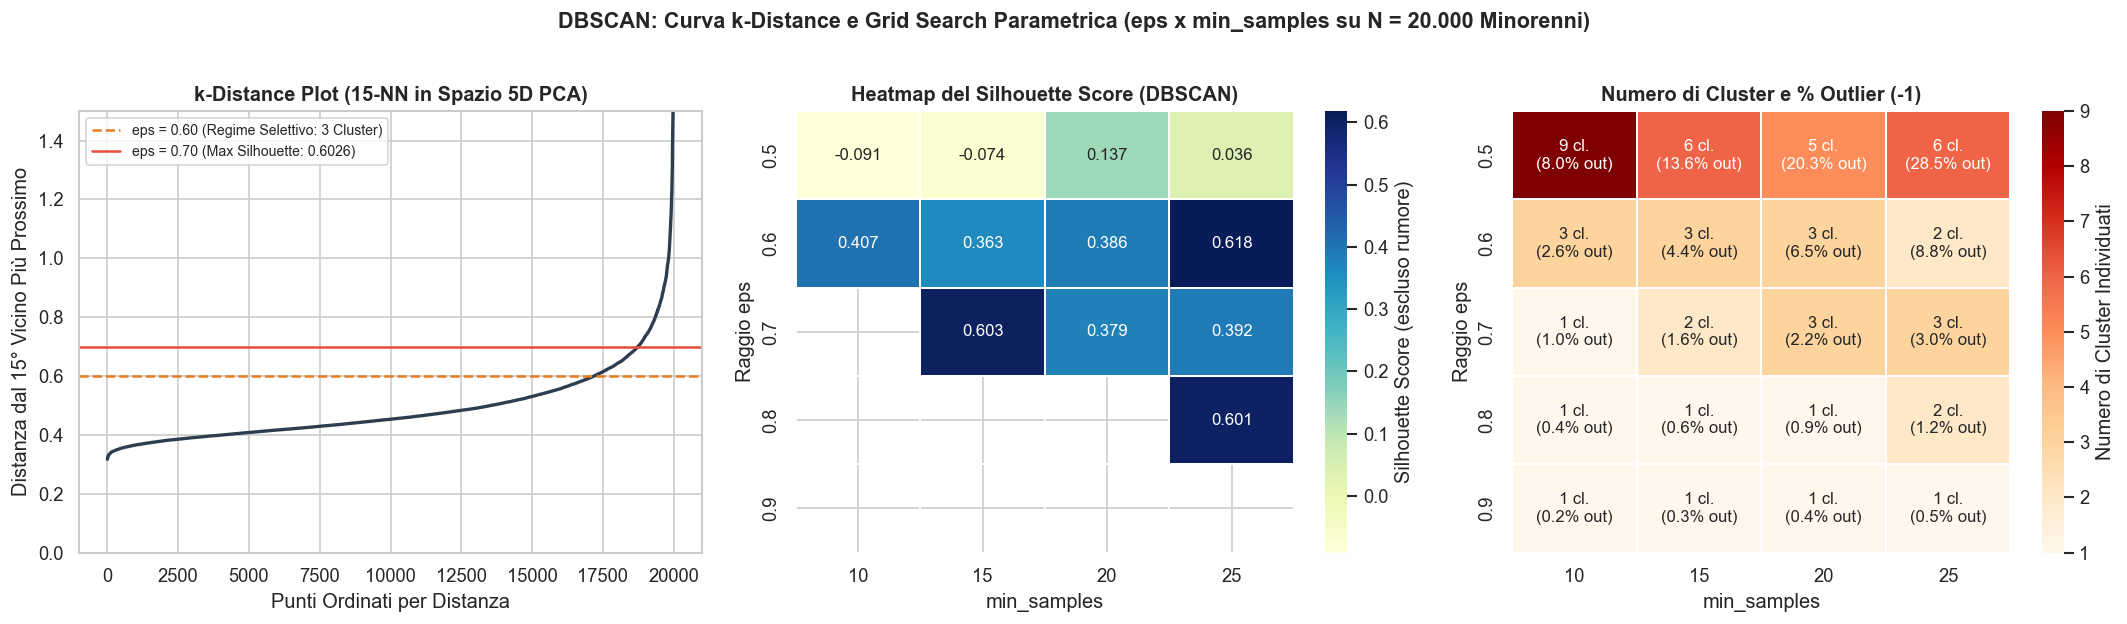
\includegraphics[width=\textwidth]{clustering/images/fig11_dbscan_kdistance_gridsearch.png}
    \caption{DBSCAN: curva $k$-Distance (a sinistra), Heatmap del Silhouette Score sui cluster validi (al centro) e Heatmap del numero di cluster e percentuale di Outlier \texttt{-1} (a destra).}
    \label{fig:dbscan_grid}
\end{figure}

\subsection{Visualizzazione Geometrica di DBSCAN e Caratterizzazione degli Outlier (\texttt{-1})}
Dalla Grid Search (Figura~\ref{fig:dbscan_grid}) emergono due regimi fondamentali:
\begin{itemize}
    \item \textbf{Regime Macro-Densità ($\varepsilon = 0,70, \text{min\_samples} = 15 \rightarrow \text{Silhouette} = \mathbf{0,6026}$):} individua \textbf{2 cluster} più l'$1,58\%$ di Outlier (\texttt{-1}), separando l'\textbf{Isola Digital Detox} ($1,74\%$) dal \textbf{Continente Principale} ($96,68\%$).
    \item \textbf{Regime Selettivo ($\varepsilon = 0,60, \text{min\_samples} = 10 \rightarrow \text{Silhouette} = \mathbf{0,4073}$):} oltre a separare il Continente Principale e l'Isola Detox, isola un \textbf{3\textsuperscript{o} Micro-Cluster Patologico Estremo (Cluster 2)} composto da minorenni con \textbf{$454,67$ minuti/giorno ($> 7,5$ ore!)}, \textbf{$46,67$ sessioni/giorno}, \textbf{Stress $34,00/40$} e \textbf{Felicità $1,67/10$}.
\end{itemize}

\begin{figure}[H]
    \centering
    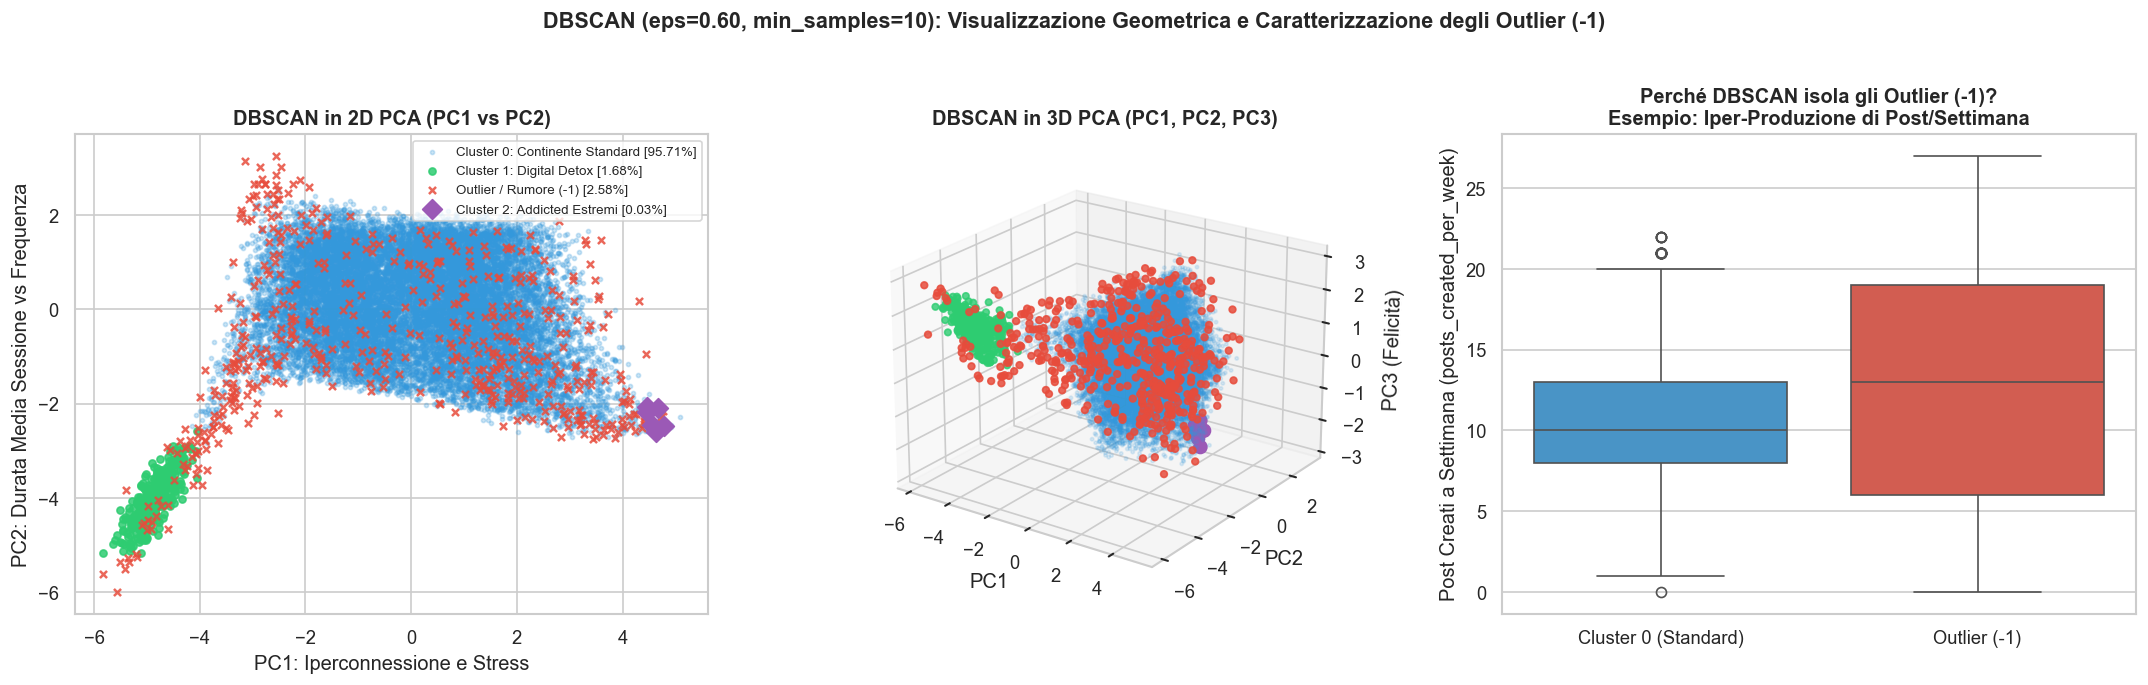
\includegraphics[width=\textwidth]{clustering/images/fig12_dbscan_2d_3d_outliers.png}
    \caption{DBSCAN ($\varepsilon=0,60, \text{min\_samples}=10$): proiezione 2D PCA, 3D PCA e caratterizzazione degli Outlier (\texttt{-1}) tramite distribuzione di \texttt{posts\_created\_per\_week}.}
    \label{fig:dbscan_viz}
\end{figure}

\begin{table}[H]
\centering
\caption{Profilazione dei Cluster e degli Outlier (\texttt{-1}) individuati da DBSCAN ($\varepsilon = 0,60, \text{min\_samples} = 10$, $N = 20.000$).}
\label{tab:dbscan_profile}
\resizebox{\textwidth}{!}{%
\begin{tabular}{lrrrrrrrrr}
\toprule
\textbf{Gruppo DBSCAN ($\varepsilon=0,60, \text{ms}=10$)} & \textbf{Conteggio} & \textbf{Quota \%} & \textbf{Minuti IG/dì} & \textbf{Sessioni/dì} & \textbf{Durata Sess.} & \textbf{Post/sett.} & \textbf{Stress (0--40)} & \textbf{Felicità (1--10)} & \textbf{Engagement} \\
\midrule
\textbf{Rumore / Outlier (\texttt{-1}): Creator e Anomalie} & 515 & 2,58\% & 182,81 & 13,30 & 18,28 m & \textbf{13,05} & 16,55 & 5,86 & \textbf{2,77} \\
\textbf{Cluster 0: Continente Principale (Standard + Intensi)} & 19.143 & 95,71\% & 227,83 & 12,37 & 21,52 m & 10,24 & 20,38 & 5,43 & 1,21 \\
\textbf{Cluster 1: Isola Digital Detox} & 336 & 1,68\% & \textbf{5,12} & 1,00 & 5,12 m & 7,67 & \textbf{2,70} & \textbf{9,11} & \textbf{10,56} \\
\textbf{Cluster 2: Micro-Cluster Patologico Estremo} & 6 & 0,03\% & \textbf{454,67} & \textbf{46,67} & 9,77 m & \textbf{16,67} & \textbf{34,00} & \textbf{1,67} & 1,01 \\
\bottomrule
\end{tabular}%
}
\end{table}

% =============================================================================
\section{Algoritmo 3 --- Clustering Gerarchico a Densità Variabile con \texttt{HDBSCAN} e Confronto Finale}
\label{sec:hdbscan}
% =============================================================================

\subsection{Applicazione di HDBSCAN: Metodo \texttt{EOM} (\emph{Excess of Mass}) contro Metodo \texttt{Leaf}}
L'algoritmo \textbf{HDBSCAN} costruisce una gerarchia di densità completa senza richiedere un raggio $\varepsilon$ fisso e consente due strategie di estrazione dall'albero condensato:
\begin{itemize}
    \item \textbf{\texttt{cluster\_selection\_method = 'eom'} (\emph{Excess of Mass}):} estrae i macro-cluster globalmente più stabili lungo l'albero gerarchico.
    \item \textbf{\texttt{cluster\_selection\_method = 'leaf'}:} estrae i nodi foglia più granulari in fondo all'albero gerarchico, individuando i \textbf{nuclei puri ad altissima densità locale} e lasciando la zona di transizione continua come rumore (\texttt{-1}).
\end{itemize}

\begin{figure}[H]
    \centering
    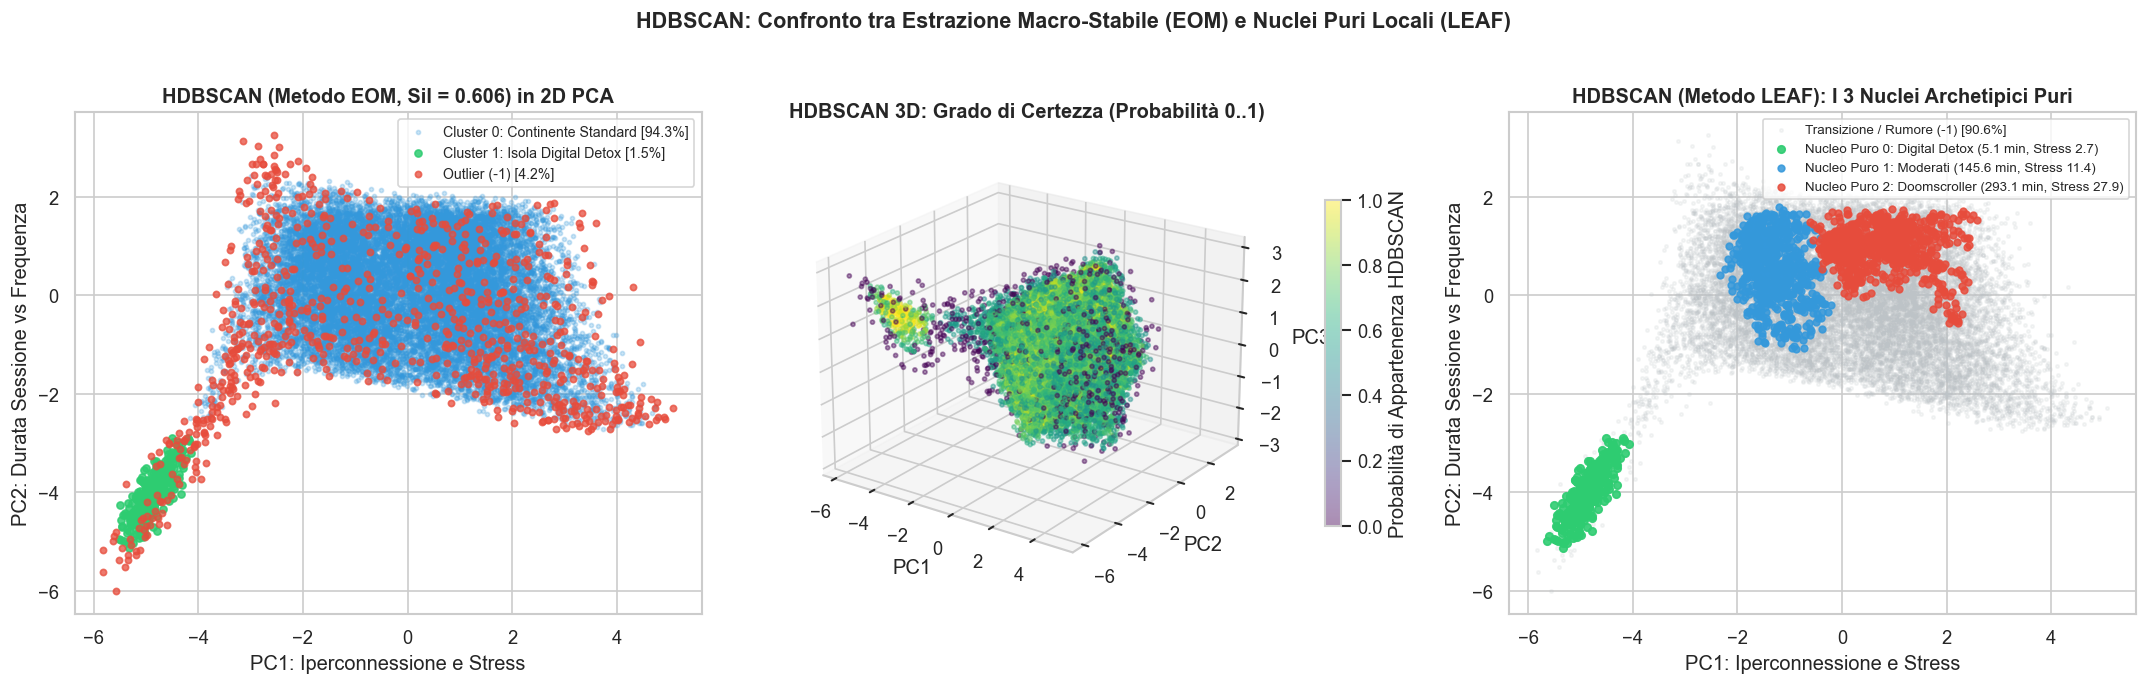
\includegraphics[width=\textwidth]{clustering/images/fig13_hdbscan_eom_vs_leaf.png}
    \caption{HDBSCAN: estrazione macro-stabile \texttt{EOM} in 2D PCA (a sinistra), grado di certezza/probabilità in 3D PCA (al centro) ed estrazione dei 3 nuclei archetipici puri tramite metodo \texttt{Leaf} (a destra).}
    \label{fig:hdbscan_viz}
\end{figure}

\begin{table}[H]
\centering
\caption{Profilazione di HDBSCAN con metodo \texttt{EOM} (\texttt{min\_cluster\_size=100, min\_samples=15}, Silhouette $= 0,6061$) e metodo \texttt{Leaf} (\texttt{min\_cluster\_size=200, min\_samples=10}, Silhouette $= 0,4512$).}
\label{tab:hdbscan_profiles}
\resizebox{\textwidth}{!}{%
\begin{tabular}{llrrrrrrrrr}
\toprule
\textbf{Metodo} & \textbf{Gruppo / Cluster HDBSCAN} & \textbf{Conteggio} & \textbf{Quota \%} & \textbf{Minuti IG/dì} & \textbf{Sessioni/dì} & \textbf{Durata Sess.} & \textbf{Post/sett.} & \textbf{Stress (0--40)} & \textbf{Felicità (1--10)} & \textbf{Engagement} \\
\midrule
\textbf{EOM} & Outlier (\texttt{-1}): Casi Limite / Creator & 642 & 3,21\% & 185,54 & 13,58 & 18,35 m & 12,51 & 16,69 & 5,86 & 2,61 \\
\textbf{EOM} & Cluster 0: Continente Principale & 19.047 & 95,24\% & 228,15 & 12,34 & 21,54 m & 10,22 & 20,40 & 5,43 & 1,19 \\
\textbf{EOM} & Cluster 1: Isola Digital Detox & 311 & 1,56\% & \textbf{5,12} & 1,00 & 5,12 m & 7,62 & \textbf{2,70} & \textbf{9,11} & \textbf{10,58} \\
\midrule
\textbf{LEAF} & Zona di Transizione Continua (\texttt{-1}) & 18.113 & 90,56\% & 226,97 & 12,73 & 21,21 m & 10,41 & 20,31 & 5,45 & 1,24 \\
\textbf{LEAF} & \textbf{Nucleo Puro 0: Digital Detox} & 311 & 1,56\% & \textbf{5,12} & 1,00 & 5,12 m & 7,62 & \textbf{2,70} & \textbf{9,11} & \textbf{10,58} \\
\textbf{LEAF} & \textbf{Nucleo Puro 1: Utenti Moderati Puri} & 777 & 3,88\% & \textbf{145,61} & 6,37 & 23,60 m & 7,82 & \textbf{11,36} & \textbf{5,98} & 1,25 \\
\textbf{LEAF} & \textbf{Nucleo Puro 2: Doomscroller Puri} & 799 & 4,00\% & \textbf{293,11} & 10,58 & 27,82 m & 10,16 & \textbf{27,93} & \textbf{5,09} & 1,04 \\
\bottomrule
\end{tabular}%
}
\end{table}

\subsection{Discussione Critica e Confronto Finale tra i 3 Algoritmi}

Il confronto incrociato tra \textbf{K-Means}, \textbf{DBSCAN} e \textbf{HDBSCAN (\texttt{EOM} e \texttt{Leaf})} fornisce una comprensione completa della topologia dei dati adolescenziali:
\begin{enumerate}
    \item \textbf{Perché DBSCAN e HDBSCAN (\texttt{EOM}) ottengono un Silhouette Score altissimo ($\sim 0,603\text{--}0,606$) ma trovano 2 soli macro-cluster?} Nello spazio 5D esiste una sola vera frattura vuota di densità: quella che separa l'isola \textbf{Digital Detox} ($\sim 5,1$ min/giorno, Stress $2,7/40$, Felicità $9,1/10$) dal resto della popolazione adolescenziale. Tra gli utenti \emph{Moderati} e i \emph{Doomscroller} esiste invece un ponte continuo di densità senza spazi vuoti.
    \item \textbf{La prova regina di HDBSCAN (\texttt{Leaf}):} Quando chiediamo a HDBSCAN di estrarre i picchi locali di densità massima (\texttt{cluster\_selection\_method = 'leaf'}, Tabella~\ref{tab:hdbscan_profiles}), l'algoritmo \textbf{ritrova esattamente i 3 archetipi di K-Means}:
    \begin{itemize}
        \item \emph{Nucleo Puro 0 (Detox):} $5,12$ min/dì, Stress \textbf{$2,70$}, Felicità \textbf{$9,11$} (K-Means Cl.0: $5,87$ min, Stress $2,81$).
        \item \emph{Nucleo Puro 1 (Moderati):} $145,61$ min/dì, Stress \textbf{$11,36$}, Felicità \textbf{$5,98$} (K-Means Cl.1: $138,70$ min, Stress $11,10$).
        \item \emph{Nucleo Puro 2 (Doomscroller):} $293,11$ min/dì, Stress \textbf{$27,93$}, Felicità \textbf{$5,09$} (K-Means Cl.2: $311,22$ min, Stress $29,07$).
    \end{itemize}
\end{enumerate}

\begin{table}[H]
\centering
\caption{Tabella riassuntiva di confronto finale tra i 3 algoritmi di Clustering analizzati.}
\label{tab:confronto_finale}
\resizebox{\textwidth}{!}{%
\begin{tabular}{p{3.4cm}p{4.3cm}p{4.3cm}p{4.3cm}}
\toprule
\textbf{Caratteristica / Metrica} & \textbf{K-Means ($k=3$ / $k=4$)} & \textbf{DBSCAN ($\varepsilon=0,60 \div 0,70$)} & \textbf{HDBSCAN (\texttt{EOM} / \texttt{Leaf})} \\
\midrule
\textbf{Paradigma Geometrico} & Partizionale basato su Centroidi (minimizza varianza WCSS) & Densità a soglia fissa ($\varepsilon, \text{min\_samples}$) & Gerarchico a densità variabile (\emph{Mutual Reachability}) \\
\addlinespace
\textbf{Numero di Cluster} & \textbf{3} (o \textbf{4} distinguendo \emph{Maratoneti} vs \emph{Compulsivi FOMO}) & \textbf{2} ($\varepsilon=0,70$) oppure \textbf{3} ($\varepsilon=0,60$, incluso micro-cluster estremo) & \textbf{2} macro-cluster (\texttt{EOM}) oppure \textbf{3} nuclei archetipici puri (\texttt{Leaf}) \\
\addlinespace
\textbf{Silhouette Score} & \textbf{0,2987} ($k=3$) / \textbf{0,2639} ($k=4$) su tutti i punti & \textbf{0,6026} ($\varepsilon=0,70$) / \textbf{0,4073} ($\varepsilon=0,60$) sui cluster validi & \textbf{0,6061} (\texttt{EOM}) / \textbf{0,4512} (\texttt{Leaf}) sui cluster validi \\
\addlinespace
\textbf{Gestione Outlier (\texttt{-1})} & Assente (forza tutti i $146.258$ minorenni in un cluster) & Eccellente ($1,58\%\text{--}2,58\%$ isolati: \emph{Creator} iper-produttivi e casi estremi) & Eccellente + fornisce \textbf{Probabilità di Appartenenza} $[0, 1]$ per ogni utente \\
\addlinespace
\textbf{Utilità Clinica per Rischio Salute Mentale (Opzione A1)} & \textbf{Massima per Stratificazione Globale:} ripartisce l'intera popolazione nelle 3 fasce di Rischio (Basso $2,2\%$, Moderato $47,2\%$, Alto $50,5\%$) & \textbf{Massima per Anomaly Detection:} isola la nicchia \emph{Digital Detox} e il micro-gruppo patologico ($>7,5$h/dì, Stress $34/40$) & \textbf{Massima per Validazione Topologica:} dimostra che i 3 profili di K-Means corrispondono ai 3 picchi di densità locale (\texttt{Leaf}) \\
\bottomrule
\end{tabular}%
}
\end{table}
